\chapter{Experiments and Results}
\label{ch:Experiments}

In this chapter we introduce all performed experiments. This includes a general experimental setup, as well as more detailed experiment settings including their results.

Since our work is twofold, we start with the experiments regarding the replication of the PGExplainer with a changed \ac{TM} architecture and a focus on the inductive setting in Section \ref{sec:experiments_replication}. Next, we describe the experiments performed on the adapted explainer framework to generate explanations for the NeuroSAT model predictions of unsatisfiable problems in Section \ref{sec:SAT-experiments}.

\section{Replication of PGExplainer}
\label{sec:experiments_replication}
In this section we present all experiments regarding the replication of the presented explainer model. We first put forward the common experimental setup, including the datasets, corresponding \acp{TM} and hyperparameter searches (see Section \ref{sec:PGE_exp_setup}). In Section \ref{sec:ind_results} we replicate the experiments in the inductive setting from the original paper with our adapted \acp{TM}. Furthermore, in Section \ref{sec:coll_exp} we perform the original quantitative experiment in the collective setting for better comparability, as this was the core study of the original paper. We also include a study on the effect of using a larger set of training data, as the original proposes that only few training instances are necessary for the explainer to generalize well (see Section \ref{sec:exp_more_train}). In Section \ref{sec:flipped_gt} we run an experiment specific to the BA-2Motif dataset, as we found that it behaves opposite to the expectations. Later, we study the effects of the specific node sets that were used in the original codebase in Section \ref{sec:motif_set_experiment}. Lastly, we qualitatively evaluate the explanations provided by our reimplemented model (see Section \ref{sec:qual_exp}).

\subsection{Common experimental setup}
\label{sec:PGE_exp_setup}
In this section we describe the common setup for the experiments that we perform on PGExplainer.
We follow the experimental setup from the PGExplainer as closely as possible. Since the textual description refers to the setup from GNNExplainer and is lacking in some aspects, we mostly extract the missing information from the codebase. As the hyperparameters are unclear or not comprehensible for some tasks we also draw information from the settings used in the replication by Holdijk et al. \cite{holdijk2021re}. \bigskip

\textbf{Datasets}\par
We perform the experiments on the same datasets used in the original. These were constructed by the authors similarly to the ones used in the baseline GNNExplainer. Four synthetic datasets were used for the node classification tasks. For the graph classification task the authors provide one synthetic dataset as well as the real-world dataset MUTAG. The synthetic datasets are constructed by creating a base graph and attaching motifs to random nodes of the base graph. These motifs determine the labels of the nodes or graphs, depending on the task at hand, and therefore serve as the \ac{GT} explanations that the explainer shall detect. Statistics of each dataset can be found in Table \ref{tab:dataset-statistics} and a visualization in Section \ref{sec:data_vis}. We will give a short description of each dataset. \bigskip

Since three of the synthetic datasets use a \ac{BA} graph as a base, we briefly introduce the BA model \cite{albert2002statistical}. The BA model generates scale-free networks that grow over time. Starting with an initialization network of $m_0 \geq m$ nodes, at each step a new node is added and connected to $m$ of the nodes already existing in the graph. The probability for each node to be selected as a neighbor depends on its degree, leading to a higher probability for nodes that already have a high degree rather than nodes with a low degree. \bigskip

BA-Shapes is the first node dataset that consists of a single BA-graph with 300 nodes and 80 house motifs - five nodes resembling the shape of a house (see Figure \ref{fig:subfig1}). Base graph nodes are labeled with 0 while nodes at the top/middle/bottom of the "house" are labeled with 1,2,3, respectively. The top node of each house motif is attached to a random base graph node. Additional edges are added for perturbation. Each node is assigned a 10-dimensional feature vector of 1s.

BA-Community consists of two unified BA-Shapes graphs. The features of the nodes are sampled from two Gaussian distributions. Nodes are labeled according to the house motif scheme for each community respectively, leading to 8 classes in total.

Tree-Cycles uses an 8-level balanced binary tree as a base graph. 80 cycle motifs, consisting of a 6 node cycle (see \ref{fig:subfig2}), are attached to random nodes from the base graph. Node features are assigned as a 10-dimensional vector of 1s. A node of the base graph is labeled as 0 and a motif node is labeled as 1.

The Tree-Grid dataset is assembled in the same way as Tree-Cycles, with the difference that the motifs are 3-by-3 grids (see \ref{fig:subfig3}). Node features and labels also follow the same procedure.

BA-2Motif is the first graph-level dataset with 800 graphs. Each of these graphs is obtained by attaching either a house or a cycle as a motif to a base BA graph of 20 nodes. According to the attached motif the graphs are assigned one of two labels, with 0 or 1 implying a house or circle, respectively.

The real-world dataset MUTAG contains $4,337$ molecule graphs that are assigned to one of 2 classes, depending on the molecules mutagenic effect \cite{riesen2008iam}, \cite{ying2019gnnexplainer}. Node features are assigned as a one-hot encoding in $\{0,1\}^{14}$, representing the chemical group of a node out of 14 possible ones. Following \cite{debnath1991structure}, \cite{ying2019gnnexplainer}, carbon rings with chemical groups $NH_2$ or $NO_2$ are known to be mutagenic, with carbon rings in general existing in both mutagenic and non-mutagenic graphs. The authors thus propose treating the carbon ring as a shared base graph and $NH_2$ and $NO_2$ as motifs for mutagenic graphs (see \ref{fig:subfig4}). Since there are no explicit motifs for the non-mutagenic graphs, these graphs are not considered in PGExplainer.

\begin{table}[h]
    \centering
    \scriptsize
    \begin{tabular}{l|cccc|cc}
    \hline
    \textbf{} & \textbf{BA-Shapes} & \textbf{BA-Community} & \textbf{Tree-Cycles} & \textbf{Tree-Grid} & \textbf{BA-2motifs} & \textbf{MUTAG} \\
    \hline
    \#graphs & 1 & 1 & 1 & 1 & 1,000 & 4,337 \\
    \#nodes  & 700 & 1,400 & 871 & 1,231 & 25,000 & 131,488 \\
    \#edges  & 4,110 & 8,920 & 1,950 & 3,410 & 51,392 & 266,894 \\
    \#labels & 4 & 8 & 2 & 2 & 2 & 2 \\
    \hline
    \end{tabular}
    \caption[Statistics of PGExplainer datasets]{Dataset statistics for Node and Graph Classification tasks, reprinted from \cite{luo2020parameterized}.}
    \label{tab:dataset-statistics}
\end{table}

Note that in the collective setting used in the original paper the explainer is trained and evaluated on the same data. This data is further reduced by only using graphs and nodes that contain a \ac{GT} motif. This makes sense for evaluation, since the AUROC cannot be calculated for \acp{GT} with only one class present. However, the authors do not specify why the training is performed only on these instances. Therefore, only the 1,015 mutagenic graphs where either $NH_2$ or $NO_2$ are present are selected for the MUTAG experiment. \bigskip

\begin{figure}[h]
    \centering
    % First 3 images
    \begin{subfigure}[b]{0.2\textwidth}
        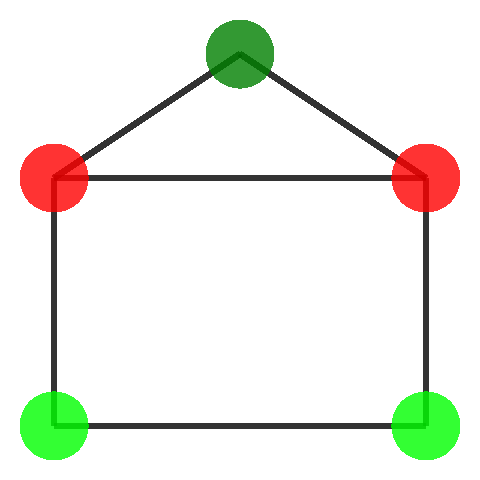
\includegraphics[width=\linewidth]{img/Motif_Vis/BA-Shapes-MOTIF.pdf}
        \caption{House motif}
        \label{fig:subfig1}
    \end{subfigure}
    \begin{subfigure}[b]{0.2\textwidth}
        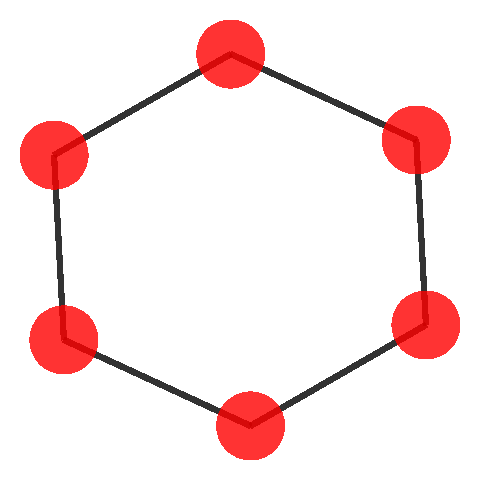
\includegraphics[width=\linewidth]{img/Motif_Vis/Tree-Cycles-MOTIF.pdf}
        \caption{Circle motif}
        \label{fig:subfig2}
    \end{subfigure}
    \begin{subfigure}[b]{0.2\textwidth}
        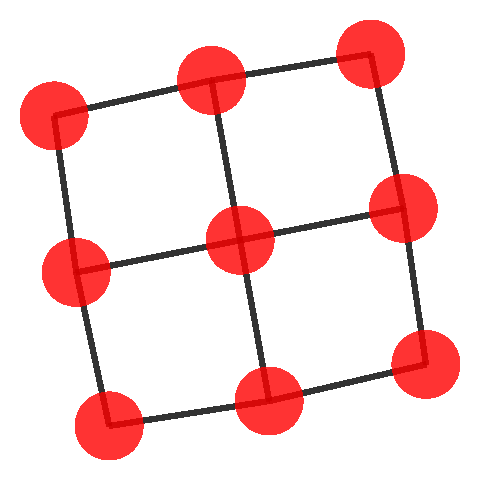
\includegraphics[width=\linewidth]{img/Motif_Vis/Tree-Grid-MOTIF.pdf}
        \caption{Grid motif}
        \label{fig:subfig3}
    \end{subfigure}
    % Fourth image composed of two smaller images
    \begin{subfigure}[b]{0.30\textwidth}
        \centering
        \begin{subfigure}[b]{0.48\linewidth}
            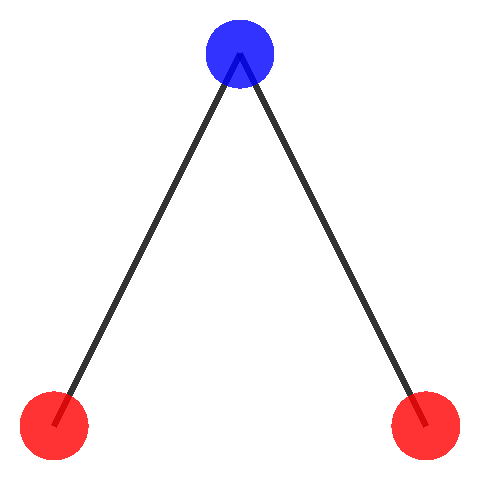
\includegraphics[width=\linewidth]{img/Motif_Vis/MUTAG-MOTIF1.pdf}
        \end{subfigure}
        \begin{subfigure}[b]{0.48\linewidth}
            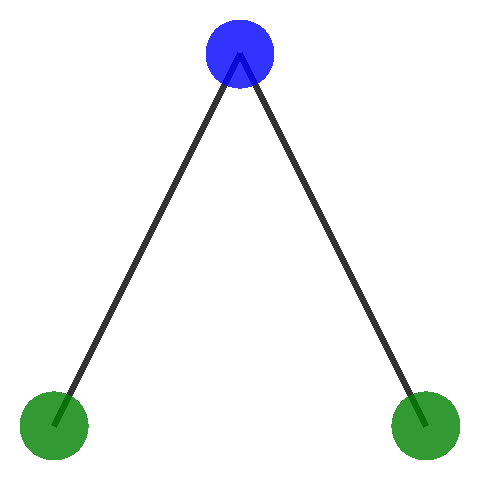
\includegraphics[width=\linewidth]{img/Motif_Vis/MUTAG-MOTIF2.pdf}
        \end{subfigure}
        \caption{$NO_2$ and $NH_2$ motifs}
        \label{fig:subfig4}
    \end{subfigure}
    
    \caption{The different motifs used in the datasets.}
    \label{fig:motifs}
\end{figure}

In the node classification experiments the instance sets $\mathcal{I}$ containing the nodes to be explained, used for both training and evaluation, were further finetuned per dataset. This leads to a selection of either all nodes that are part of a motif, or only one node per motif. This inconsistency is also left unexplained by the authors and extracted from the codebase. It is likely adapted from the GNNExplainer \cite{ying2019gnnexplainer}, where single-instance and multi-instance explanations are differentiated. We perform an experiment on the effects of these node selections in \ref{sec:motif_set_experiment}.

For the instance set $\mathcal{I}$ used in BA-community multiple configurations exist in the PGExplainer codebase. One is extracted from the GNNExplainer \cite{ying2019gnnexplainer} and consists of the same nodes used for the BA-Shapes dataset, which seems unjustified and is not addressed in the paper. Another setting uses all motif nodes of both communities - effectively all nodes that do not belong to the two community base graphs. We select this setting for our replication, as this makes more sense than using the arbitrary indices from BA-Shapes. \bigskip

The selection of instances for the remaining dataset is as follows: In BA-Shapes one "middle" node from each motif in the graph is selected as instance. A similar selection is used in Tree-Cycles, where the "first" motif node connected to the base graph is chosen for each motif. For Tree-Grid all motif nodes in the graph are selected as instances, similar to BA-Community. For the graph dataset BA-2Motif all graphs are used as instances, since each one explicitly contains one of the two motifs. The consequential number of instances $N$ used for each dataset are listed in Table \ref{tab:motif-statistics}. Note that these instance sets are only considered in the explainer and not during \ac{TM} training.

\begin{table}[h]
    \centering
    \scriptsize
    \begin{tabular}{l|cccc|cc}
    \hline
    \textbf{} & \textbf{BA-Sh.} & \textbf{BA-Co.} & \textbf{Tree-Cy.} & \textbf{Tree-Gr.} & \textbf{BA-2M.} & \textbf{MUTAG} \\
    \hline
    \#total motif instances & 300 & 800 & 360 & 289 & 1,000 & 1,015 \\
    \#used motif instances $N$ & 60 & 800 & 60 & 289 & 1,000 & 1,015 \\
    \hline
    \end{tabular}
    \caption[Statistics of motif instances per dataset]{Amount of possible and actually used motif instances per dataset, as found in the original codebase.}
    \label{tab:motif-statistics}
\end{table}



The fixed \ac{TM} that we use for each dataset is trained as described in Section \ref{sec:Replication_of_PGExplainer}. Since we use a different GNN layer, we try to achieve accuracies above 85\%, similar to the original. The accuracies can be seen in Table \ref{tab:our-dt-accuracy} and are slightly higher than in the original for four of the datasets, except for BA-Community and MUTAG. We add a dropout layer with a probability of $p=0.1$ to the latter two models to improve their generalizability and achieve testing scores closer to the original. The exact downstream task accuracies achieved in PGExplainer \cite{luo2020parameterized} can be seen in Table \ref{tab:compact-accuracy}. \bigskip

\begin{table}[h]
    \centering
    \scriptsize
    \begin{tabularx}{\linewidth}{l|X X X X|X X}
    \hline
    \textbf{Accuracy} & \textbf{BA-Shapes} & \textbf{BA-Community} & \textbf{Tree-Cycles} & \textbf{Tree-Grid} & \textbf{BA-2Motif} & \textbf{MUTAG} \\
    \hline
    \textbf{Training}   & 1.00 & 0.92 & 1.00 & 0.99 & 1.00 & 0.86 \\
    \textbf{Validation} & 1.00 & 0.87 & 1.00 & 0.99 & 1.00 & 0.86 \\
    \textbf{Testing}    & 0.97 & 0.89 & 0.99 & 0.99 & 1.00 & 0.82 \\
    \hline
    \end{tabularx}
    \caption[Accuracies of adapted GNN downstream task]{Accuracy table for Node and Graph Classification downstream tasks from our reimplementation using a slightly adapted GNN.}
    \label{tab:our-dt-accuracy}
\end{table}
\newpage
\textbf{Evaluation Metrics}\par
Following Luo et al. \cite{luo2020parameterized}, the explanation problem is considered a binary classification of edges for quantitative evaluation. Edges that appear in a motif are positive targets, and negative otherwise. The edge importance weights of each explained instance are treated as prediction scores.

Since the original paper does not specify the exact calculation of the AUROC score, we use the approach described in Section \ref{sec:Replication_of_PGExplainer} for a standardized procedure. Thus, we conduct the mean over the local AUROC scores of all instances as the metric for quantitative evaluation. Node instances with a local computation graph of only motif nodes are skipped in the calculation due having only positive targets. We calculate the mean local AUROC on the training-, validation and test sets individually. The validation set is used to evaluate the hyperparameter search, while the results of the following inductive experiments usually consider the score on the test set. For the collective setting we only consider a singular instance set that is used for both training and evaluation. \bigskip

To qualitatively evaluate the explanations we visualize the top-$k$ explanation mask edges with the highest prediction scores, following Luo et al. \cite{luo2020parameterized}. The parameter $k$ for each dataset is extracted from the original codebase, and is set to include at least the number of \ac{GT} motif edges in the explanation. For node classification tasks the visual explanations only include the nodes inside the local computation graph of the prediction node, as only these are relevant for the prediction \cite{ying2019gnnexplainer}. \bigskip

We perform the efficiency evaluation as described by Holdijk et al. \cite{holdijk2021re}. The average inference time needed to generate an explanation for any instance is calculated over the test set for each run individually (see Section \ref{sec:Replication_of_PGExplainer}). We include the mean of these averages for the inductive replication experiment only. \bigskip

\textbf{Hyperparameter Search}\par
Most details on the training procedure of the explainer have been established in Section \ref{sec:Replication_of_PGExplainer}. As found by Holdijk et al. \cite{holdijk2021re} the PGExplainer is very sensitive to hyperparameter settings on each dataset. Therefore, we conduct hyperparameter searches for the explainer model on each of the datasets to obtain the best performing explainers. We follow Liashchynskyi and Liashchynskyi \cite{liashchynskyi2019grid} to perform grid searches over the parameter space that we define as an extended combination of the setting used in the original \cite{luo2020parameterized}, as well as the configs provided in Replication study \cite{holdijk2021re}. 

For our hyperparameters $\lambda_1,\lambda_2,...,\lambda_n$ we define corresponding sets $S_1,S_2,...,S_n$ of possible values. The grid search finds the best model with respect to the mean of the local ROC-AUC scores of all validation instances over all combinations $(\lambda_1,\lambda_2,...,\lambda_n) \in S_1\times S_2 \times...\times S_n$. Additionally, we consider that the predicted edge importance scores shall not be exactly 0 or 1 for all edges. Since we found that some datasets behave unexpectedly regarding the evaluation metric, we may choose to optimize in the opposite direction, which we will further discuss in Section \ref{sec:ind_results}. All experiments and training were conducted on an AMD Ryzen 7 2700X processor. \bigskip

The hyperparameters tested consist of the learning rate $\eta \in \mathbb{R}^+$, the number of epochs $E \in \mathbb{N}$ used to train the explainer, the number of sampled graphs $K \in \mathbb{N}$, the initial and final temperatures $\tau_0, \tau_T \in \mathbb{R}^+$, as well as two coefficients $\alpha_e\in \mathbb{R}^+$ and $\alpha_s\in \mathbb{R}^+$ to control the entropy regularization and the size regularization, respectively. For the BA-Community explainer we also test a sample bias $b=0.5$, that restricts the $\epsilon$ in Equation \ref{eq:reparam_trick} to $\epsilon \sim \text{Uniform}(0+b,1-b)$. This is also extracted from the original codebase and leads to a constant $\epsilon=0.5$. We further define a set of fixed seeds used during each grid search as $S=\{74,75,76\}$, since we found that the performance of the explainer is highly dependent on the seed for some of the datasets. \bigskip

Since we care about the inductive performance and Luo et al. \cite{luo2020parameterized} demonstrate that the explainer performs well on few training instances, we set the number of training instances $a=30$ for graph tasks and $a=0.08$ for node tasks during the searches. We choose a percental split for the node tasks, since the node sets used in the original experiment highly vary in size and generally contain fewer instances than the graph sets. The resulting absolute number of training instances for the node tasks, as well as the specifics of each search can be seen in Section \ref{sec:sweeps}. Following PGExplainer \cite{luo2020parameterized}, the resulting validation set and test set each have a size of $\frac{(N-a)}{2}$, where $N$ denotes the number of used instances in each dataset. The optimal hyperparameter values used for the following experiments are listed in Table \ref{tab:best_sweep_values}. \bigskip

\begin{table}[h]
    \centering
    \scriptsize
    \begin{tabular}{|c|c|c|c|c|c|c|c|c|} \hline
    Dataset & $K$ & $b$ & $E$ & $\eta$ & $\alpha_e$ & $\alpha_s$ & $\tau_0$ & $\tau_T$ \\ \hline
    \textbf{BA-Shapes} & 1 & 0.0 & 10 & 0.003 & 0.1 & 0.05 & 5.0 & 1.0 \\ \hline
    \textbf{BA-Community} & 5 & 0.0 & 20 & 0.003 & 1.0 & 0.1 & 1.0 & 5.0 \\ \hline
    \textbf{Tree-Cycles} & 5 & 0.0 & 20 & 0.0003 & 1.0 & 0.0001 & 1.0 & 1.0 \\ \hline
    \textbf{Tree-Grid} & 5 & 0.0 & 30 & 0.003 & 1.0 & 0.5 & 5.0 & 2.0 \\ \hline
    \textbf{BA-2Motif} & 10 & 0.0 & 20 & 0.01 & 0.1 & 0.03 & 5.0 & 1.0 \\ \hline
    \textbf{MUTAG} & 10 & 0.0 & 20 & 0.01 & 1.0 & 0.005 & 5.0 & 1.0 \\ \hline
    \end{tabular}
    \caption[Optimal explainer parameter values for each dataset]{The best-performing parameter values for each dataset based on the performed grid searches (see Section \ref{sec:sweeps}).}
    \label{tab:best_sweep_values}
  \end{table}

\textbf{Baselines}\par
 We compare our work to both the collective and inductive results from the original PGExplainer paper, as well as the results from the collective PyTorch replication study by Holdijk et al. \cite{holdijk2021re} (see Table \ref{tab:pgexplainer_baseline}). Since the inductive results of PGExplainer are only provided as plots, we approximate the numeric values. \bigskip

\begin{table}[ht]
    \centering
    \scriptsize
    \begin{tabularx}{\textwidth}{lXXXX|XX}   % 'X' column type from tabularx automatically scales columns
    \textbf{} & \multicolumn{4}{c}{\textbf{Node Classification}} & \multicolumn{2}{c}{\textbf{Graph Classification}} \\
    \textbf{Method} & BA-Shapes & BA-Community & Tree-Cycles & Tree-Grid & BA-2Motif & MUTAG \\
    \midrule
    \addlinespace
    \textbf{} & \multicolumn{6}{c}{\textbf{Explanation AUROC}} \\
    \midrule
    PGExplainer & 0.963$\pm$0.011 & 0.945$\pm$0.019 & 0.987$\pm$0.007 & 0.907$\pm$0.014 & 0.926$\pm$0.021 & 0.873$\pm$0.013 \\
    \midrule
    RE-PGExplainer & 0.999$\pm$0.000 & 0.825$\pm$0.040 & 0.760$\pm$0.014 & 0.679$\pm$0.008 & 0.133$\pm$0.046 & 0.843$\pm$0.084 \\
    \midrule
    PGExplainer (inductive) & $\sim$0.98 & $\sim$0.99 & $\sim$0.99 & $\sim$0.88 & $\sim$0.84 & - \\
    \midrule
    \addlinespace
    \textbf{} & \multicolumn{6}{c}{\textbf{Inference Time (ms)}} \\
    \midrule
    \textit{PGExplainer} & 10.92 & 24.07 & 6.36 & 6.72 & 80.13 & 9.68 \\
    \textit{RE-PGExplainer} & 3.58 & 5.23 & 0.45 & 0.54 & 0.33 & 2.05 \\
    \bottomrule
    \end{tabularx}
    \caption[Baseline PGExplainer and RE-PGExplainer]{PGExplainer performance baselines.}
    \label{tab:pgexplainer_baseline}
\end{table}


\textbf{Experimental Protocol}\par
We follow the general experimental setup used in the baselines \cite{luo2020parameterized}, \cite{holdijk2021re}, originally proposed in \cite{ying2019gnnexplainer}. We train a PGExplainer model on a fixed \ac{TM} with a specified seed, with the hyperparameter values listed in Table \ref{tab:best_sweep_values}. This process is repeated 10 times for each dataset. The models are evaluated quantitatively using the AUROC metric and qualitatively for select experiments, in the sense of comparing visualizations of explanations to the \ac{GT} motifs. We provide the quantitative results as the mean and standard deviation over 10 runs for all experiments. \bigskip


\subsection{Inductive Setting}
\label{sec:ind_results}

\textbf{Experimental Setup} \par
In this experiment we evaluate the quantitative performance of PGExplainer in the inductive setting on our slightly adapted \acp{TM}. Since Luo et al. \cite{luo2020parameterized} showed that the PGExplainer can achieve good results with only few training instances, we aim to replicate this for $a=30$ training instances, one of the original experiment settings. Since the exact instances used are not further specified in the paper, we treat the motif node sets described in Section \ref{sec:PGE_exp_setup} as the instance sets of size $N$ for node task.

We repeat this experiment with Xavier \cite{glorot2010understanding} used as initialization for the explainer MLP weights, opposed to the He \cite{he2015delving} initialization standard to PyTorch linear layers with ReLU activations. This is done since the grid searches showed that the performance is heavily dependent on the used seed for some datasets, which mainly controls the initializations. Xavier is used by default in the original TensorFlow \cite{tensorflow2015-whitepaper} implementation.

Additionally, we measure the average inference time to explain any instance and compare it to both baselines. \bigskip

%NOTE: Tree-Grid with original experimental setup (all motif nodes, 30 training instances) leads to mean of 0.5 for almost all hyperparam settings tried. Size reg of 0.05 (as in original) leads to all edges being assigned a values of one!

\textbf{Results}\par
Table \ref{tab:pgexplainer_auc} shows the quantitative results, as well as the inference time for all dataset. First, BA-Shapes is the only experiment that comes close to the originally recorded scores. It is notable, that both Tree-Cycles and BA-2Motif achieve an AUROC score far below $0.5$, indicating that the opposite of the \ac{GT} expectations is predicted. Though the variance of Tree-Cycles is quite high, the figures \ref{fig:Tree-Cycles-val_loss} and \ref{fig:Tree-Cycles-val_auroc} show that this is mostly cause by a singular outlier run. Both the losses and AUROC scores are decreasing steadily, illustrating a stable learning process. 

\begin{figure}[htbp]
    \centering
    \begin{subfigure}[b]{0.48\textwidth}
        \centering
        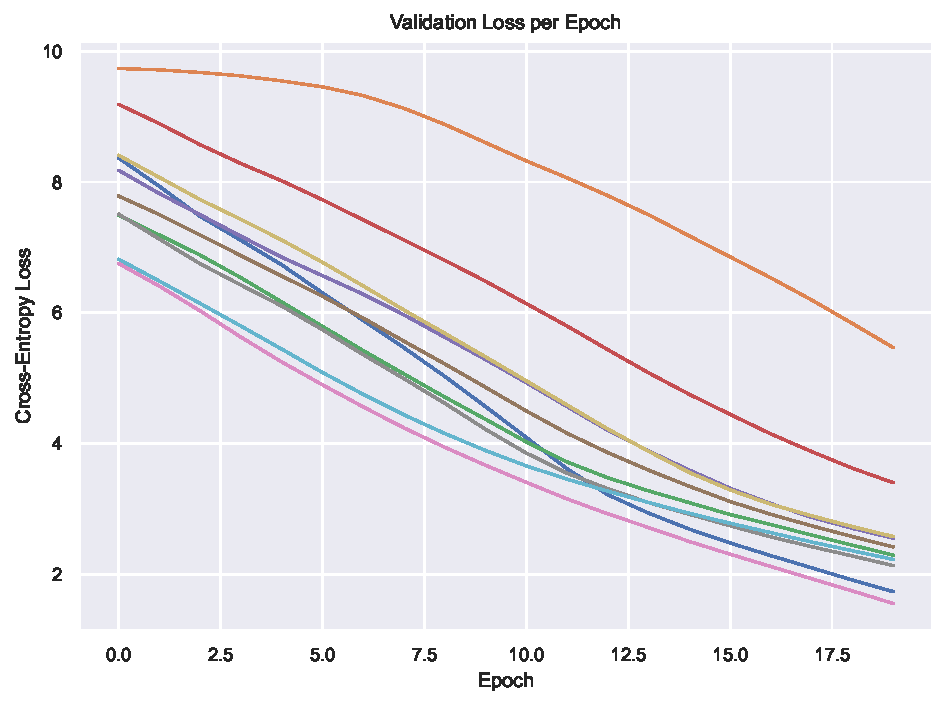
\includegraphics[width=\textwidth]{img/plots/Cycles_val_loss_plot_NO_LEGEND.pdf}
        \caption{Mean validation Loss}
        \label{fig:Tree-Cycles-val_loss}
    \end{subfigure}
    \hfill
    \begin{subfigure}[b]{0.48\textwidth}
        \centering
        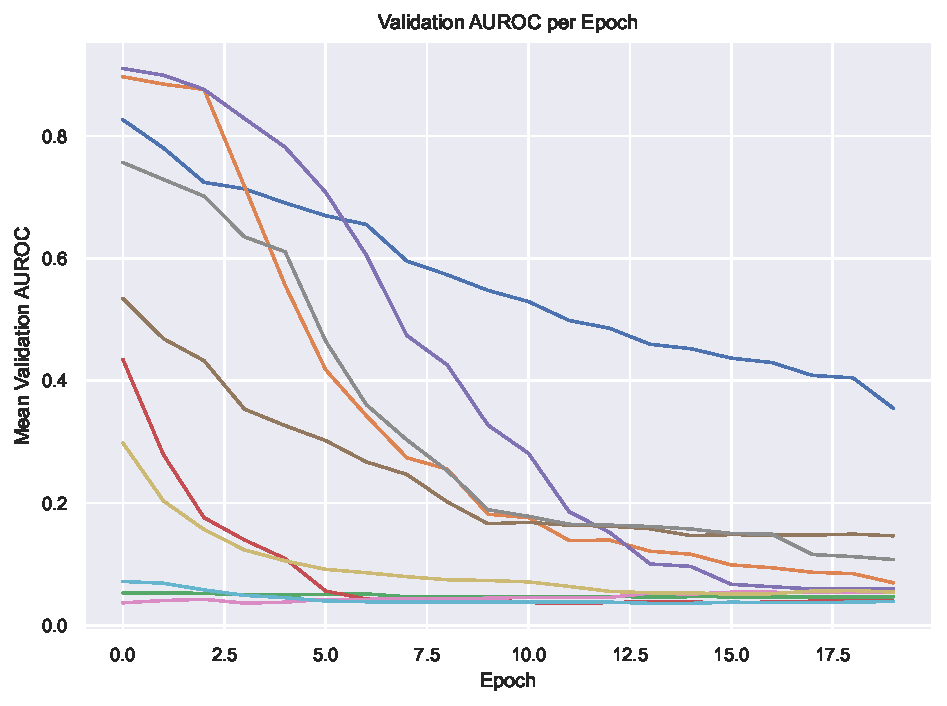
\includegraphics[width=\textwidth]{img/plots/Cycles_val_auroc_plot_NO_LEGEND.pdf}
        \caption{Mean validation AUROC}
        \label{fig:Tree-Cycles-val_auroc}
    \end{subfigure}
    \caption[Validation metrics for Tree-Cycles]{Validation metrics for Tree-Cycles over 10 runs in inductive setting.}
    \label{fig:Tree-Cycles-val_metrics}
\end{figure}

We were unable to determine a reason for the unexpected opposite classification of select tasks, but highlight that this can also be observed for BA-2Motif in the replication study \cite{holdijk2021re} (see Table \ref{tab:pgexplainer_baseline}). To validate this, we perform an experiment with flipped \ac{GT} edges in Section \ref{sec:flipped_gt}. \bigskip

\begin{table}[ht]
    \centering
    \scriptsize
    \begin{tabularx}{\textwidth}{l|XXXX|XX}   % 'X' column type from tabularx automatically scales columns
    \textbf{} & \multicolumn{4}{c}{\textbf{Node Classification}} & \multicolumn{2}{c}{\textbf{Graph Classification}} \\
    \textbf{Method} & BA-Shapes & BA-Community & Tree-Cycles & Tree-Grid & BA-2Motif & MUTAG \\
    \midrule
    \addlinespace
    \textbf{} & \multicolumn{6}{c}{\textbf{Explanation AUROC}} \\
    \midrule
    PGExplainer & $\sim$0.98 & $\sim$0.99 & $\sim$0.99 & $\sim$0.88 & $\sim$0.84 & - \\
    \midrule
    Our work (He) & 0.994$\pm$0.001 & 0.754$\pm$0.013 & 0.106$\pm$0.104 & 0.537$\pm$0.081 & 0.017$\pm$0.006 & 0.874$\pm$0.009 \\
    \midrule
    Our work (Xavier) & 0.995$\pm$0.002 & 0.779$\pm$0.036 & 0.467$\pm$0.316 & 0.551$\pm$0.119 & 0.035$\pm$0.05 & 0.834$\pm$0.04 \\
    \midrule
    \addlinespace
    \textbf{} & \multicolumn{6}{c}{\textbf{Inference Time (ms)}} \\
    \midrule
    \textit{PGExplainer} & 10.92 & 24.07 & 6.36 & 6.72 & 80.13 & 9.68 \\
    \textit{RE-PGExplainer} & 3.58 & 5.23 & 0.45 & 0.54 & 0.33 & 2.05 \\
    \textit{Our work} & 37.0$\pm$1.4 & 24.8$\pm$0.1 & 3.0$\pm$0.2 & 2.7$\pm$0.1 & 4.0$\pm$0.3 & 4.0 \\
    \bottomrule
    \end{tabularx}
    \caption[Inductive performance of our reimplementation]{Inductive performance of PGExplainer ($a=30$).}
    \label{tab:pgexplainer_auc}
\end{table}

When considering that AUROC scores close to 0 also indicate learning, Tree-Grid is the worst performing dataset, converging to a metric score close to random guessing. We note that the loss does converge as expected in all runs, but the model seems to be unable to generalize well.

It is notable that the Xavier initialized model achieves worse results across the board. Though the mean values are higher for most of the datasets, the variance is also much higher, suggesting less stability. Since we care for stable models we only consider He initialization for the following experiments. \bigskip

Our implementation improves the inference time of the explainer for 4 datasets, but is notably slower for BA-Shapes. We report considerably lower times than the replication study, which we primarily attribute to our limited hardware.


%We use normalization in our \acp{TM}, though it is not described in the paper, since it is used in the code. We also experimented with the effects of the use of normalization since it seems to be relevant to the performance of the explainer. \\

%It is important to highlight that our code achieved better and way more stable results for BA-2Motif when trained on a gpu instead of cpu. \\
%Ba-Shapes, Tree-Cycles and MUTAG results achieved were identical. \\
%Ba-Community and Tree-Grid achieved very slightly better results on CPU. \\

%Sweeps: (Params ordered by importance)\\
%BA-Shapes: higher size reg -> 0.1; lower entropy reg -> 0.01; lr and tT very low impact but slightly higher -> 0.01 and 5. Note that Loss curve jumps on most runs! (logical-sweep-94 and restful-sweep-92 have clean loss) TRY HIGHER SIZE REG AND LOWER ENTROPY REG \\

%BA-Community: lr 0.0001 too low, not working -> 0.003; lower entropy -> 0.1; higher size -> 0.1; TRY MORE SEEDS, LR, EPOCHS? \\

%Tree-Cycles: high lr -> 0.01 ; lower entropy reg -> 0.1/0.01; higher size reg -> 0.1/0.01 ; lower tT -> 1. TRY WITH MORE SEEDS FOR ENT, SIZE, TEMP? Confirmed higher size reg -> 0.1; lower entropy reg -> 0.01; temp really low impact, tendency higher. TRY 30 EPOCHS???\\

%Tree-Grid: high lr -> 0.01; high size reg -> 1; higher entropy reg? -> 10/1, high tT -> 5. TRY MORE SEEDS FOR ENTROPY REG -> not quite clear, tendency lower; MAYBE EVEN HIGHER LR -> No\\

%BA-2Motif: RUN ON GPU - Not the cause. Cause for better results were features of 1 instead of 0.1! However, good results achieved on BA2-Motif dataset from pyg, not original one.\\

%MUTAG: Low lr -> 0.0003; low entropy reg(high impact, but highest AUC runs vary) -> 0.1; low tT -> 1; less epochs -> 20; low size reg -> 0.005(/0.01); Loss is messy and AUC seems to decrease over time! lr 0.0001 worse, entropy reg 0.1/0.01 has zero effect -> 0.1\\

\subsection{Collective Setting}
\label{sec:coll_exp}

\textbf{Experimental Setup} \par
To allow for a better comparison with both baselines we perform an experiment in the collective setting. Therefore, both the training and evaluation are performed on the complete set of motif instances. This is the setting that can be found in the original codebase. It is noteworthy that we use the hyperparameters found in an inductive setting (see Section \ref{sec:PGE_exp_setup}), which should allow for good generalization. We also include our results obtained in the inductive setting, to evaluate the difference between the settings. \bigskip

\textbf{Results}\par

We are unable to reproduce the scores achieved in the original work for most of the datasets, as seen in Table \ref{tab:pgexplainer_auc_collective}. BA-Shapes achieves a higher score than the original, while MUTAG comes close to the original baseline and even obtains a higher score in the inductive setting. The other scores do not come close when considering the scores as they are without flipped \acp{GT}. We are however able to match the results achieved in the replication baseline in all but the Tree-Cycles experiment. This validates that the PGExplainer achieves similar results for different target GNN layers.

\begin{table}[ht]
    \centering
    \scriptsize
    \begin{tabularx}{\textwidth}{l|XXXX|XX}   % 'X' column type from tabularx automatically scales columns
    \textbf{} & \multicolumn{4}{c}{\textbf{Node Classification}} & \multicolumn{2}{c}{\textbf{Graph Classification}} \\
    \textbf{Method} & BA-Shapes & BA-Community & Tree-Cycles & Tree-Grid & BA-2Motif & MUTAG \\
    \midrule
    \addlinespace
    \textbf{} & \multicolumn{6}{c}{\textbf{Explanation AUROC}} \\
    \midrule
    PGExplainer & 0.963$\pm$0.011 & 0.945$\pm$0.019 & 0.987$\pm$0.007 & 0.907$\pm$0.014 & 0.926$\pm$0.021 & 0.873$\pm$0.013 \\
    \midrule
    RE-PGExplainer & 0.999$\pm$0.000 & 0.825$\pm$0.040 & 0.760$\pm$0.014 & 0.679$\pm$0.008 & 0.133$\pm$0.046 & 0.843$\pm$0.084 \\
    \midrule
    Our work & 0.993$\pm$0.001 & 0.831$\pm$0.009 & 0.084$\pm$0.078 & 0.679$\pm$0.032 & 0.018$\pm$0.004 & 0.833$\pm$0.006 \\
    \midrule
    %collective with Xavier & 0.993.$\pm$0.003 & 0.833$\pm$0.023 & 0.322$\pm$0.278 & 0.68$\pm$0.057 & 0.027$\pm$0.009 & 0.774$\pm$0.034 \\
    %\midrule
    \midrule
    Our work (inductive) & 0.994$\pm$0.001 & 0.754$\pm$0.013 & 0.106$\pm$0.104 & 0.537$\pm$0.081 & 0.017$\pm$0.006 & 0.874$\pm$0.009 \\
    \bottomrule
    \end{tabularx}
    \caption[Collective performance of our reimplementation]{Collective PGExplainer performance ($a=N$).}
    \label{tab:pgexplainer_auc_collective}
\end{table}


\subsection{Inductive Setting with more training data}
\label{sec:exp_more_train}

\textbf{Experimental Setup}\par
Luo et al. \cite{luo2020parameterized} show that the inductive performance of PGExplainer improves with the number of instances used for training. To validate this we perform an inductive experiment with an increased number of training instances $a=60$. Since the motif instance sets of BA-Shapes and Tree-Cycles in the original setting only consist of 60 instances, we use a split ratio of $80/10/10$. This leads to $a=48$ for these two tasks. \bigskip

\textbf{Results}\par
The results for this experiment are found in Table \ref{tab:experiment_60train}. The graph tasks see a slight improvement, while the node tasks all seem to perform worse with more training instances. While the variance decreases for both tree tasks, the mean moves toward the value indicating random predictions. We observe that BA-Community reaches a peak in AUROC early but steadily decreases afterward, as opposed to the setting with $a=30$ where the AUROC rises steadily and converges strongly. This result suggests that the hyperparameters have to be retuned for this setting, which hinders the generalizability of the explainer. We are unable to confirm that the PGExplainer generally achieves better results when more instances are seen during training.

\begin{table}[ht]
    \centering
    \scriptsize
    \begin{tabularx}{\textwidth}{l|XXXX|XX}   % 'X' column type from tabularx automatically scales columns
    \textbf{} & \multicolumn{4}{c}{\textbf{Node Classification}} & \multicolumn{2}{c}{\textbf{Graph Classification}} \\
    \textbf{Method} & BA-Shapes & BA-Community & Tree-Cycles & Tree-Grid & BA-2Motif & MUTAG \\
    \midrule
    \addlinespace
    \textbf{} & \multicolumn{6}{c}{\textbf{Explanation AUROC}} \\
    \midrule
    Our work (inductive) & 0.994$\pm$0.001 & 0.754$\pm$0.013 & 0.106$\pm$0.104 & 0.537$\pm$0.081 & 0.017$\pm$0.006 & 0.874$\pm$0.009 \\
    \midrule
    $a=60$ & 0.987$\pm$0.002 & 0.641$\pm$0.045 & 0.144$\pm$0.096 & 0.495$\pm$0.052 & 0.017$\pm$0.004 & 0.895$\pm$0.009 \\
    \bottomrule
    \end{tabularx}
    \caption[Inductive performance with more training instances]{Inductive PGExplainer performance with more training instances where $a$ is either 48 or 60.}
    \label{tab:experiment_60train}
\end{table}

\subsection{BA-2Motif with Inverted Ground Truth}
\label{sec:flipped_gt}

\textbf{Experimental setup}\par
Since we found that the AUROC score for BA-2Motif decreases rather than increases over the training epochs, while converging near zero, we run an additional experiment with inverted  GT. Since both the loss and AUROC curves decrease steadily and flatten in the original inductive experiment (see Figure \ref{fig:BA-2Motif-val_metrics}), we consider this experiment an additional validation.
The mean individual AUROC is calculated identical to before, but the \ac{GT} mask of each graph is inverted, meaning that edges in the motif now carry a label of $0$ and all other edges a label of $1$. 
Note that the \ac{GT} does not affect the training procedure in any way and merely changes the metric evaluation. \bigskip

\begin{table}[ht]
    \centering
    \scriptsize
    \begin{tabularx}{0.45\textwidth}{l c}
        \toprule
        \textbf{Method} & \textbf{Explanation AUROC} \\
        \midrule
        PGExplainer       & 0.926$\pm$0.021 \\
        RE-PGExplainer       & 0.133$\pm$0.046 \\
        Our work       & 0.017$\pm$0.006 \\
        \midrule
        Inverted GT     & 0.985$\pm$0.006 \\
        \bottomrule
    \end{tabularx}
    \caption[Inductive performance on BA-2Motif with inverted \ac{GT}]{Explanation AUROC for BA-2Motif with inverted GT.}
    \label{tab:flippedGT}
\end{table}
\textbf{Results} \par

As expected, the AUROC score for BA-2Motif is nearly perfect in this experiment, even surpassing the original baseline, as seen in Table \ref{tab:flippedGT}. It is notable that the results by Holdijk et al. \cite{holdijk2021re} suggest a similar observation, however the authors do not expand on this.


\begin{figure}[htbp]
    \centering
    \begin{subfigure}[b]{0.48\textwidth}
        \centering
        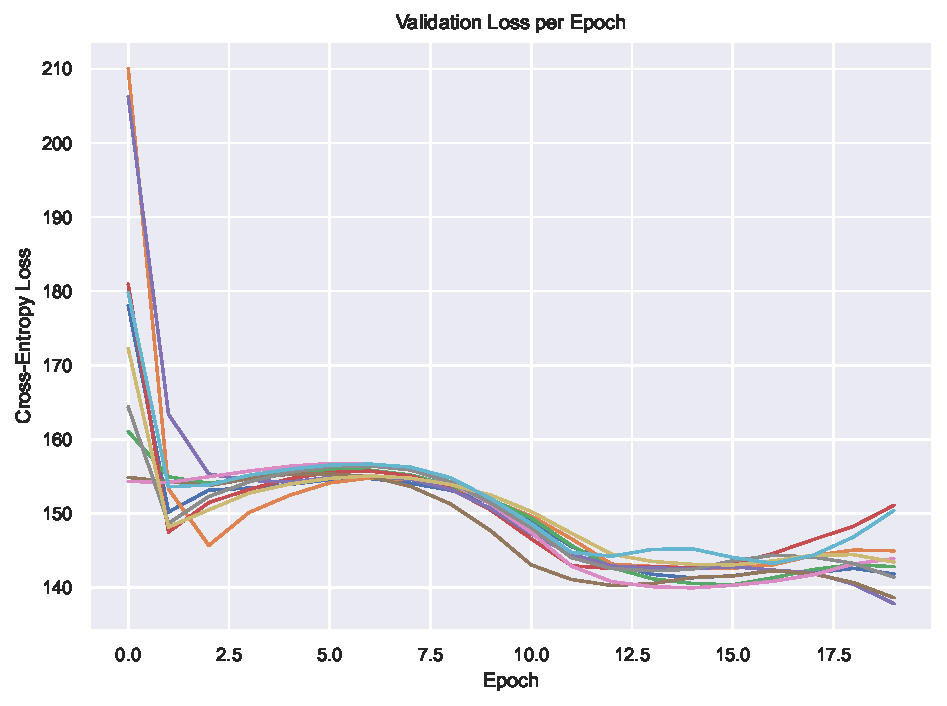
\includegraphics[width=\textwidth]{img/plots/2M_val_loss_plot_NO_LEGEND.pdf}
        \caption{Mean validation Loss}
        \label{fig:BA-2Motif-val_loss}
    \end{subfigure}
    \hfill
    \begin{subfigure}[b]{0.48\textwidth}
        \centering
        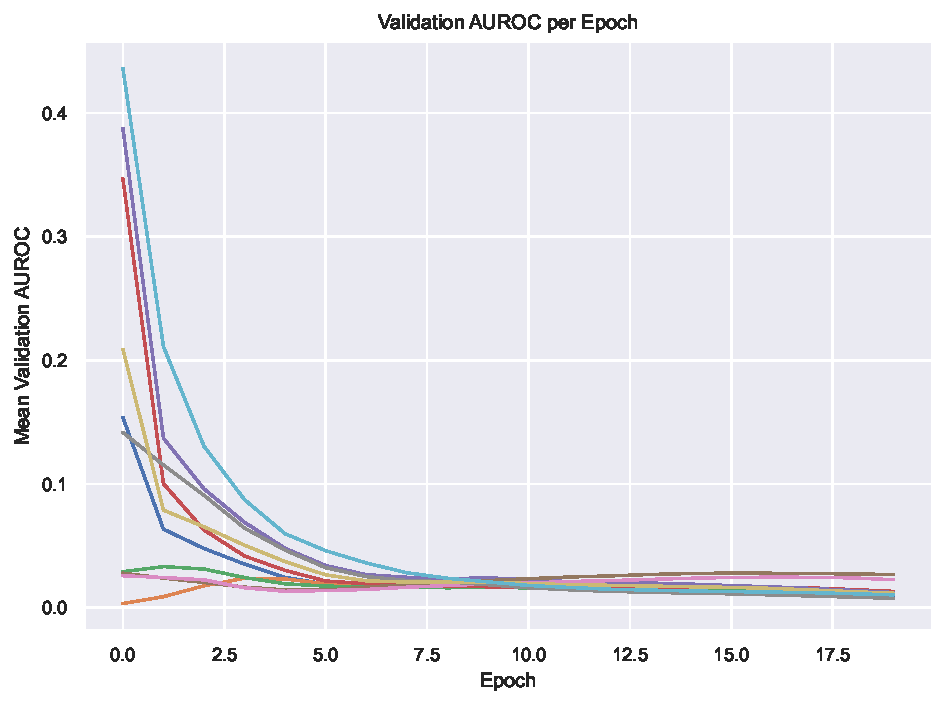
\includegraphics[width=\textwidth]{img/plots/2M_val_auroc_plot_NO_LEGEND.pdf}
        \caption{Mean validation AUROC}
        \label{fig:BA-2Motif-val_auroc}
    \end{subfigure}
    \caption[Validation metrics for BA-2Motif]{Validation metrics for BA-2Motif over 10 runs in inductive setting.}
    \label{fig:BA-2Motif-val_metrics}
\end{figure}

\subsection{Effects of Used Motif Instances for Node Tasks}
\label{sec:motif_set_experiment}

%Tree-Grid: DURING OUR TRAINING: 11 of 30 training instances consisted of only motif nodes/edges, resulting in an incomputable AUROC
%USAGE OF ALL MOTIF NODES LEADS TO k-HOP GRAPHS THAT DO NOT CONTAIN COMPLETE MOTIF! LEADS TO EXPLANATION ONLY CONTAINING 3 "BOXES" OF THE 4, AS SEEN IN BAD PERFORMING MODELS?
\textbf{Experimental Setup} \par
As presented in \ref{sec:PGE_exp_setup} the motif instances used in PGExplainer \cite{luo2020parameterized} for different node level explanation tasks do not follow the same rules. This is likely related to their direct comparison to GNNExplainer \cite{ying2019gnnexplainer} and the adaptation of their dataset settings. However, since the PGExplainer claims to generalize well and be able to provide explanations for any downstream GNN task, a uniform procedure for providing explanations is necessary. 

Evidently, different nodes in a motif have different local computation graphs, containing different motif- and non-motif nodes. The 3-hop graph computed from a corner node of a grid motif may for example never contain the complete motif. If such a node is commonly selected during training, it is reasonable to believe that the explainer may learn the "sub-motif" consisting of three squares, rather than the complete motif. A 3-layer GNN may therefore not be ideal for learning the grid motif. We evaluate the effect of using all motif nodes or a singular node from each motif as instances in this experiment.

We suggest changing the instance sets $\mathcal{I}$ for training and evaluation to include either all or one select motif node, depending on the dataset. We use the same hyperparameters used for the previous experiments. Besides this change, we follow the general experimental setup in the inductive setting with $a=30$ to evaluate whether a reasoning behind the node selection can be made out. \bigskip

Since BA-Shapes and Tree-Cycles originally use a singular node from each motif, we evaluate the effect of using all nodes in each motif and refer to this as All-Motif-Nodes. Accordingly, we select one fixed node from each motif for the BA-Community and Tree-Grid tasks, similar to the original BA-Shapes and Tree-Cycles task. For BA-Community we choose one of the two "middle" nodes in the house motif, similar to BA-Shapes. For Tree-Grid we select the "second" node, starting from the corner node attached to the base graph, as the 3-hop graph from this node contains all motif nodes as well as the most nodes from the base graph. We call this experiment One-Motif-Node. The exact number of instances used in this experiment can be seen in Table \ref{tab:motif-statistics-exp}.

It is noteworthy that using singular corresponding topological nodes across motifs restricts the explanation task in terms of generalizability, since only the explanations of these nodes are learned. %Thus, we additionally evaluate the effect of training on a subset of the singular motif nodes and evaluating on a subset of all motif nodes, to test whether the explainer is able to generalize its learned explanations to other nodes from the same motif. We call this One-Motif-Node-Train. For all datasets we select a training set of size $a$ from the singular motif node sets with size $N$ (see Table \ref{}). However, we create the validation and evaluation 


\begin{table}[h]
    \centering
    \scriptsize
    \begin{tabular}{l|cc|cc}
    \textbf{} & \multicolumn{2}{c|}{\textbf{All-Motif-Nodes}} & \multicolumn{2}{c}{\textbf{One-Motif-Node}} \\
    \addlinespace
    \toprule
    \textbf{} & \textbf{BA-Sh.} & \textbf{Tree-Cy.} & \textbf{BA-Co.} & \textbf{Tree-Gr.} \\
    \midrule
    \#total motif instances & 300 & 360 & 800 & 289 \\
    \#used motif instances $N$ & 300 & 360 & 160  & 32 \\
    \end{tabular}
    \caption[Statistics of adapted Motif Node Instance]{Amount of possible and actually used motif instances in the experiments with adapted instance sets.}
    \label{tab:motif-statistics-exp}
\end{table}

\textbf{Results}\par
We present the results of the All-Motif-Nodes experiment compared to our results achieved in the inductive setting in Table \ref{tab:allmotifnodes_selected} and for One-Motif-Node in Table \ref{tab:onemotifnode_selected}. It is most notable that the Tree-Grid experiment achieves perfect edge classification accuracy in the One-Motif-Node experiment. BA-Community also reports a significant increase in AUROC score.

The All-Motif-Nodes experiment leads to a slight deterioration in score for BA-Shapes, which is still better than the scores achieved on the other node tasks in our inductive experiment. The explainer's performance on Tree-Cycles deteriorates in both variance and mean score, particularly in terms of its distance from a random AUROC score.

\begin{table}[ht]
    \centering
    \scriptsize
    \begin{tabularx}{0.6\textwidth}{l*{2}{X}}   % Adjust width as needed
    \toprule
    \textbf{} & \multicolumn{2}{c}{\textbf{Explanation AUROC}} \\
    \cmidrule{2-3}
    \textbf{Method} & BA-Shapes & Tree-Cycles \\
    \midrule
    Our work & 0.994$\pm$0.001 & 0.106$\pm$0.104 \\
    \midrule
    AllMotifNodes & 0.959$\pm$0.004 & 0.204$\pm$0.162 \\
    \bottomrule
    \end{tabularx}
    \caption[Inductive performance using all motif nodes for training]{Explanation AUROC for All-Motif-Nodes.}
    \label{tab:allmotifnodes_selected}
\end{table}

\begin{table}[ht]
    \centering
    \scriptsize
    \begin{tabularx}{0.6\textwidth}{l*{2}{X}}   % Adjust width as needed
    \toprule
    \textbf{} & \multicolumn{2}{c}{\textbf{Explanation AUROC}} \\
    \cmidrule{2-3}
    \textbf{Method} & BA-Community & Tree-Grid \\
    \midrule
    Our work & 0.754$\pm$0.013 & 0.537$\pm$0.081 \\
    \midrule
    OneMotifNode & 0.951$\pm$0.007 & 1.0$\pm$0.0 \\
    \bottomrule
    \end{tabularx}
    \caption[Inductive performance using one motif node for training]{Explanation AUROC for One-Motif-Node .}
    \label{tab:onemotifnode_selected}
\end{table}


\subsection{Qualitative Analysis}
\label{sec:qual_exp}

\textbf{Experimental setup}\par
For the qualitative analysis the best performing explainer model for each \ac{TM} is selected, and random explanations are sampled. For the explainer models with AUROC scores below 0.5, we select the model that achieves the lowest score and visualize the top-$k$ lowest edges accordingly. Following the approach of the original, we present instance explanations that highlight the successful detection of motifs. We additionally include sample grids of 16 random graphs in the Appendix.

Following Luo et al. \cite{luo2020parameterized}, we select dataset-specific values of $k$: BA-Shapes, BA-Community and Tree-Cycles use $k=6$; Tree-Grid uses $k=12$; BA-2Motif uses $k=5$ and MUTAG uses $k=10$. \bigskip

\textbf{Results}\par
The visualized explanations generated for each \ac{TM} show that the \ac{GT} motifs are detected (see Figure \ref{fig:qual_expl}).
We found that the MUTAG explainer detects the chemical combinations that cause the mutagenicity as the highest edges regularly, but the shared base carbon ring is not detected at all. More qualitative samples for each dataset can be seen in Appendix \ref{sec:grid_vis}. The qualitative explanations of BA-Community rarely contain all connected motif edges, as seen in Figure \ref{fig:grid-BA-Community-explanations}. Note that due to the setting of $k=5$ for BA-2Motif the house motif is never detect completely, but it is clearly visible that the added house edge is detected.

\begin{figure}[h]
    \centering
    % First 3 images
    \begin{subfigure}[b]{0.15\textwidth}
        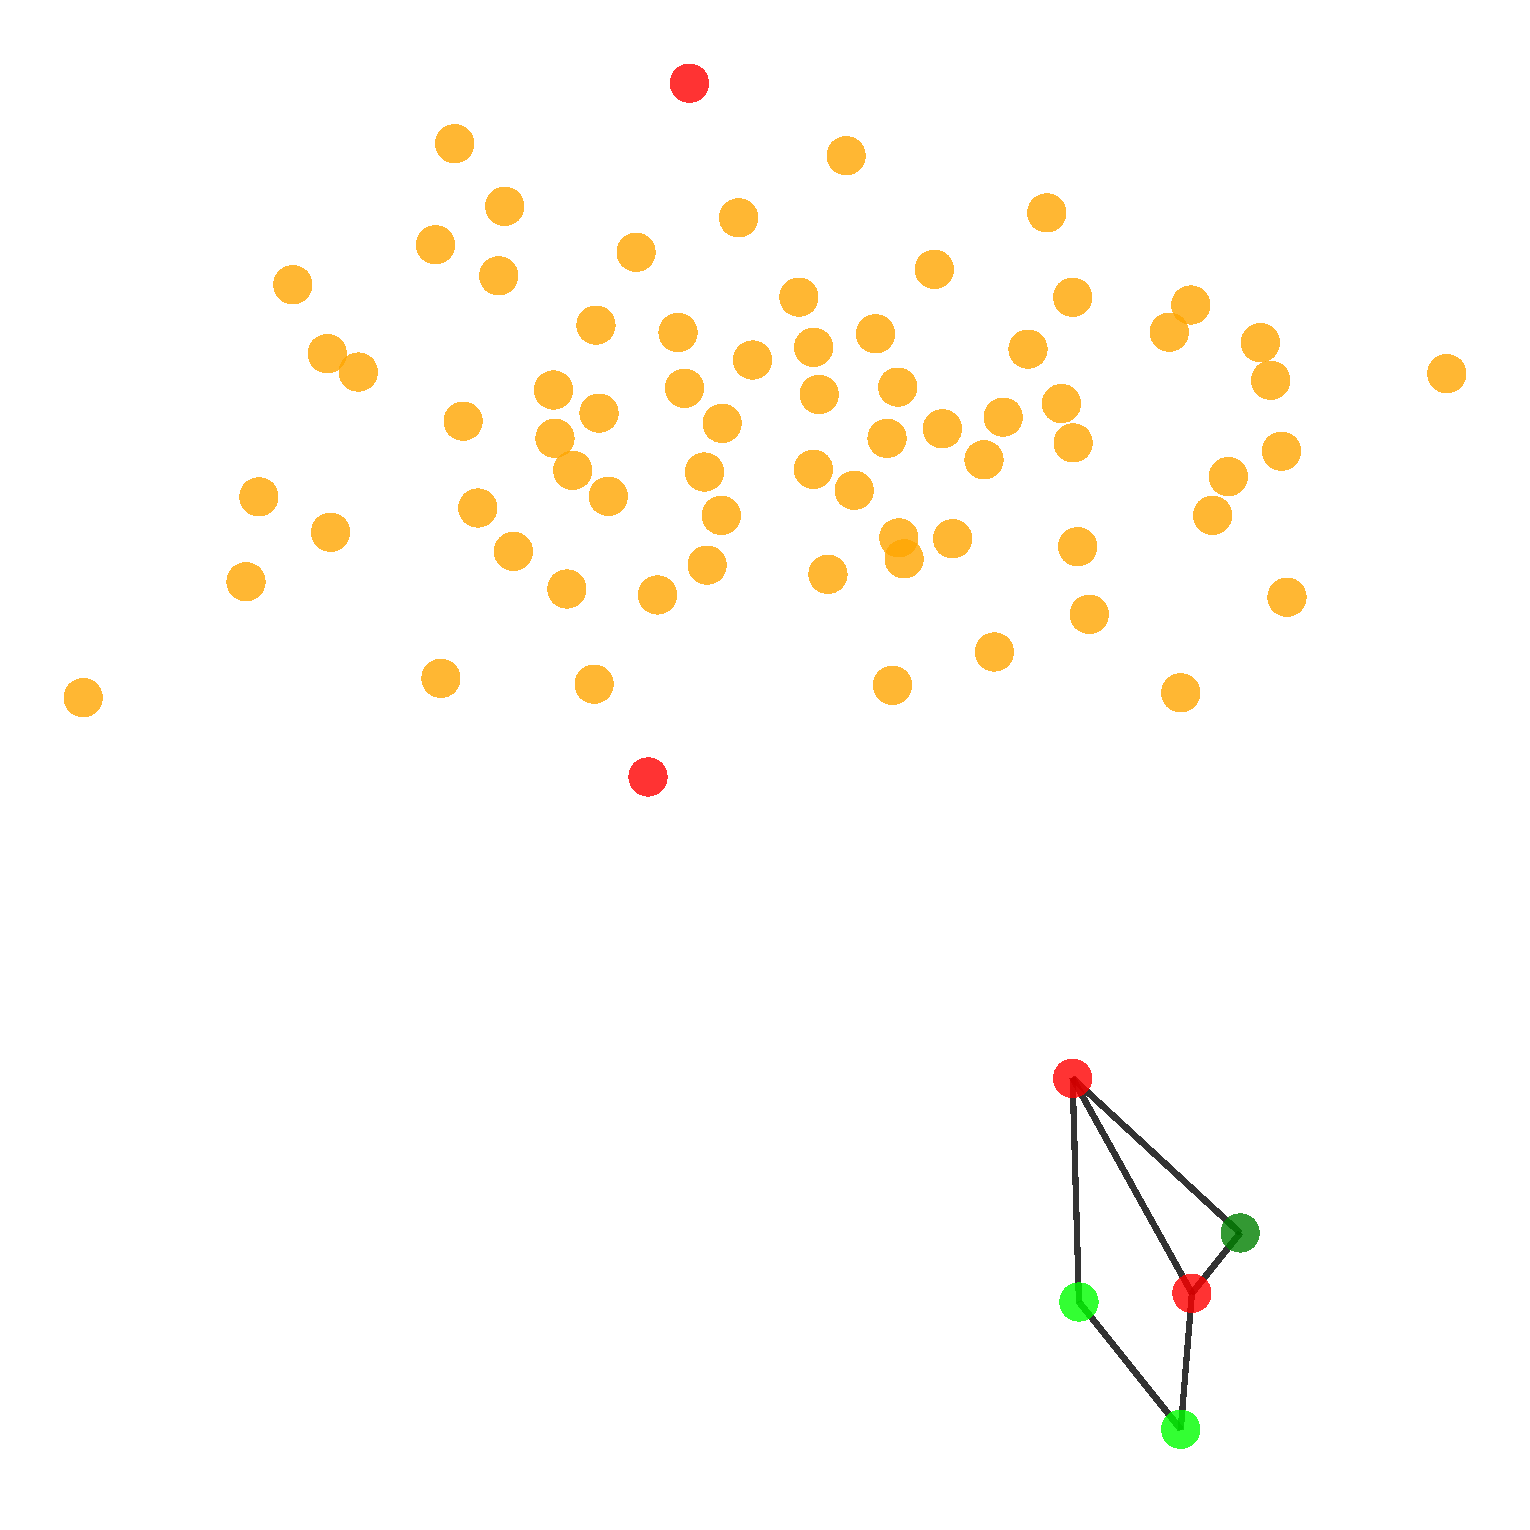
\includegraphics[width=\linewidth]{img/BA-Shapes/graph_3_explanation.pdf}
        \caption{\scriptsize BA-Sh.}
        \label{fig:qual_shapes}
    \end{subfigure}
    \begin{subfigure}[b]{0.15\textwidth}
        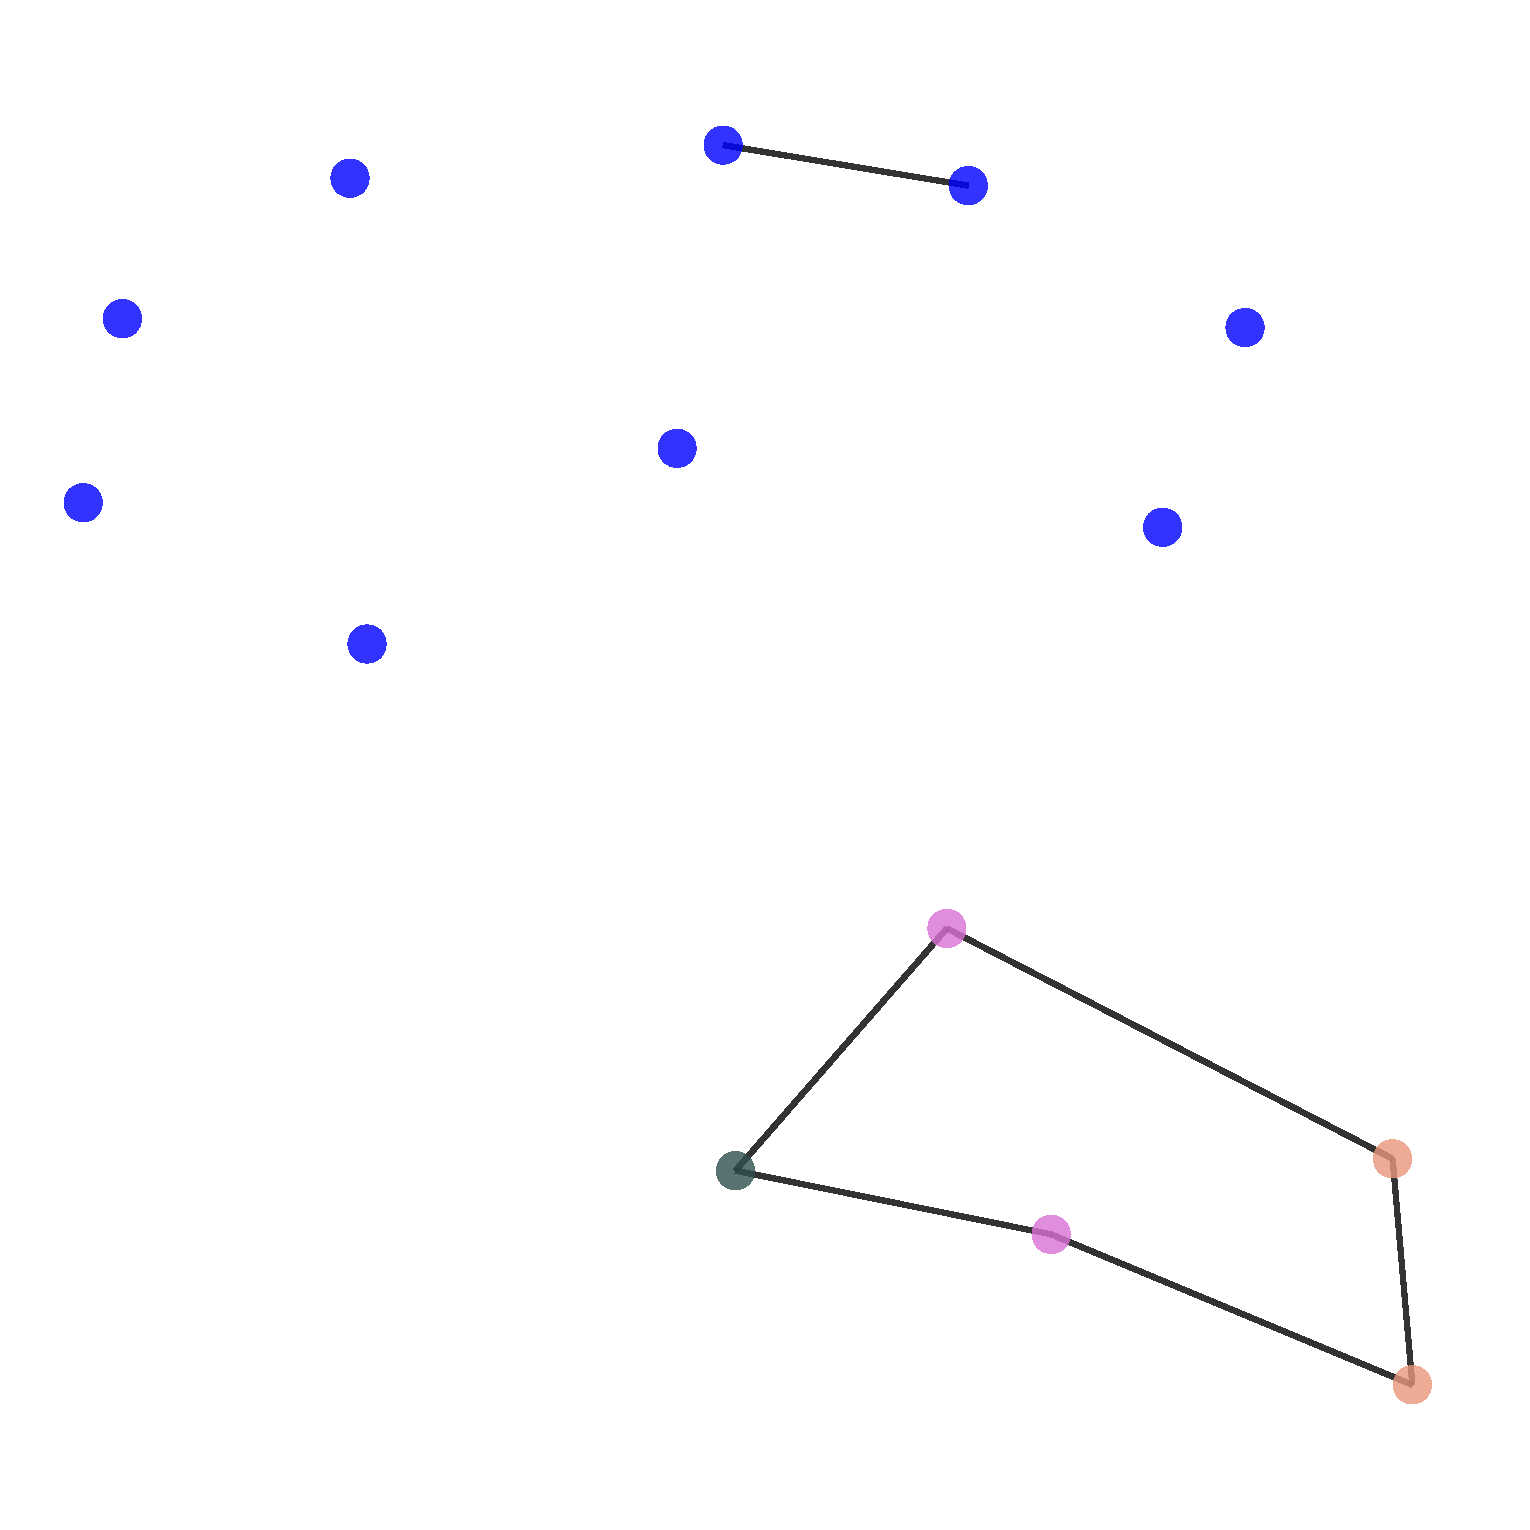
\includegraphics[width=\linewidth]{img/BA-Community/graph_11_explanation.pdf}
        \caption{\scriptsize BA-Co.}
        \label{fig:qual_comm}
    \end{subfigure}
    \begin{subfigure}[b]{0.15\textwidth}
        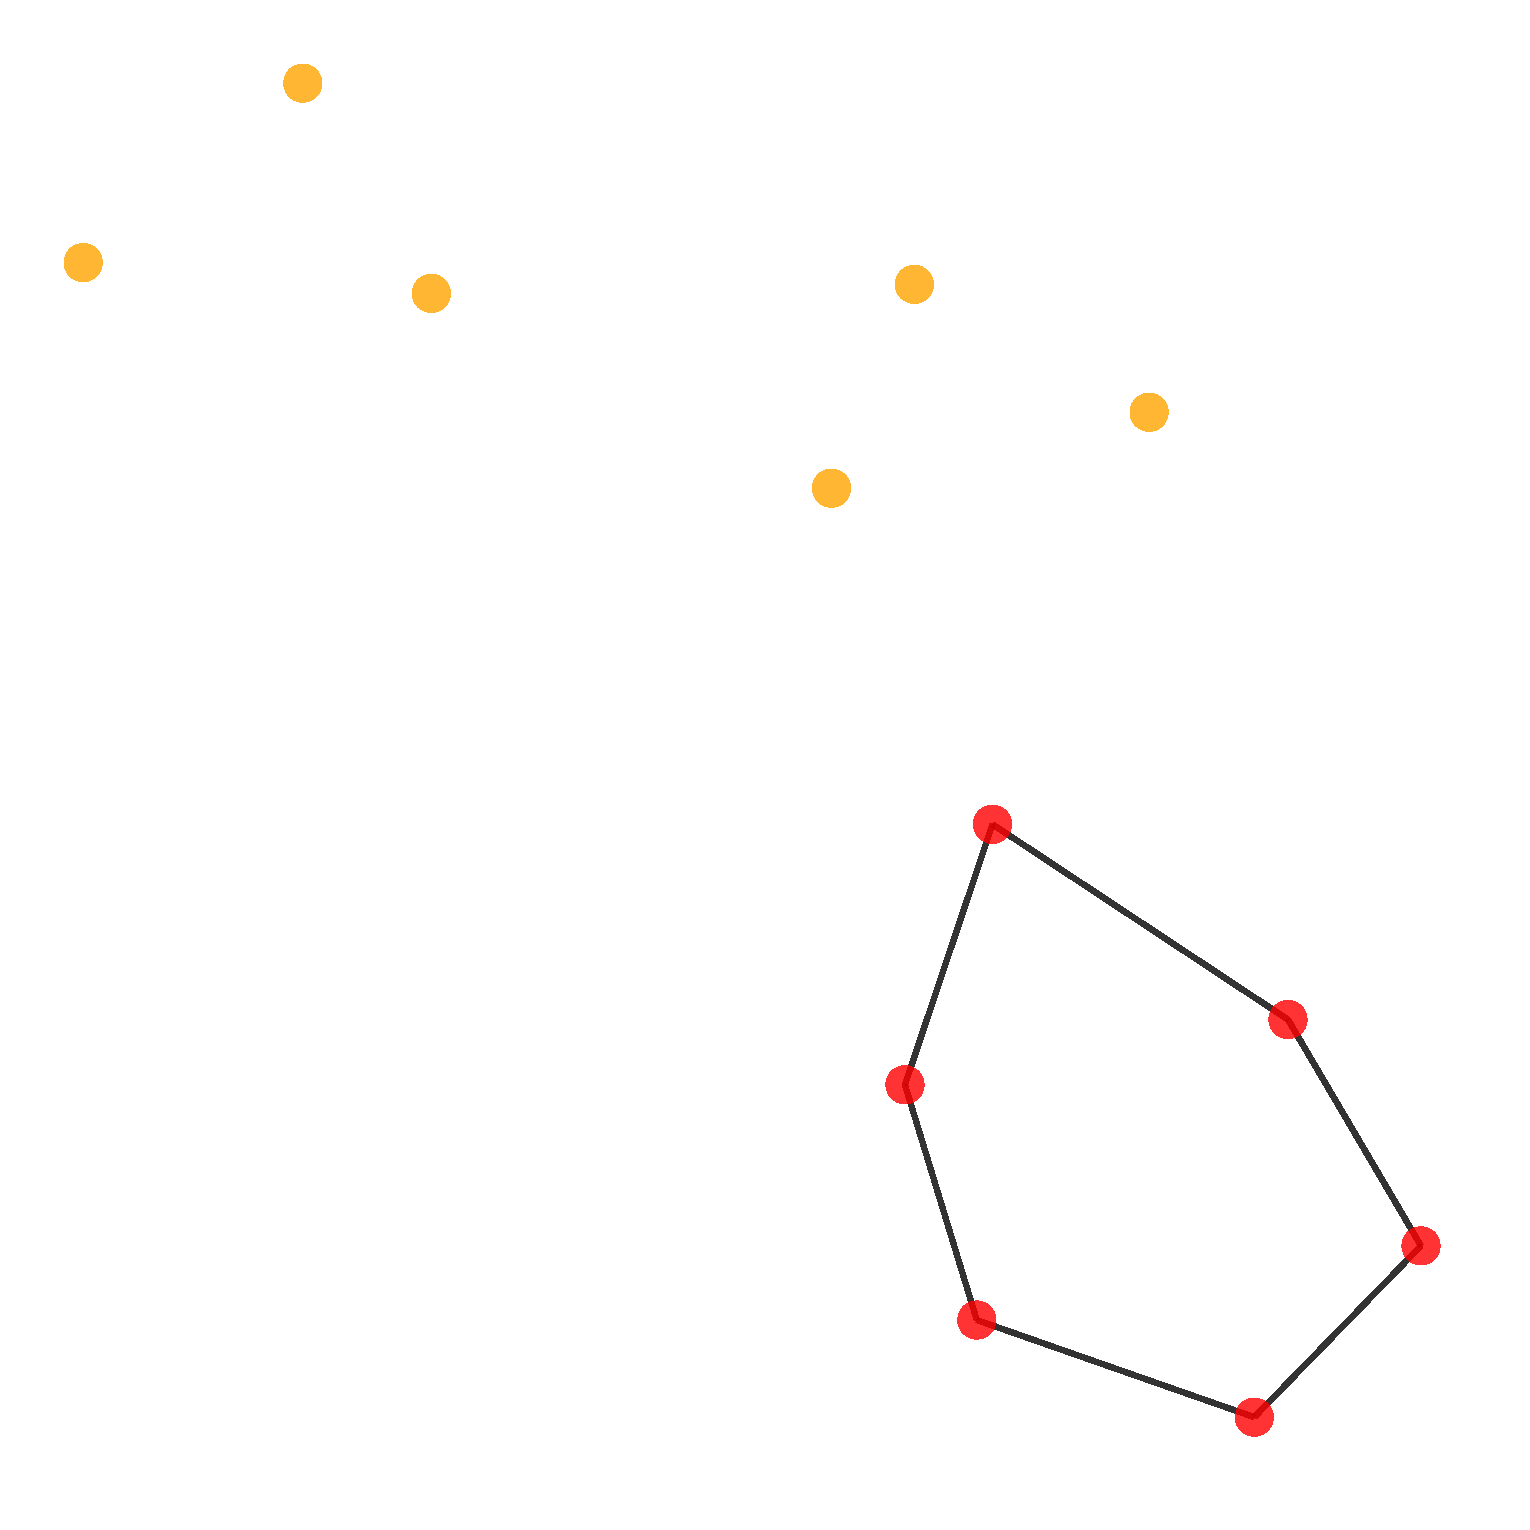
\includegraphics[width=\linewidth]{img/Tree-Cycles/graph_4_explanation.pdf}
        \caption{\scriptsize Tree-Cy.}
        \label{fig:qual_cycle}
    \end{subfigure}
    \begin{subfigure}[b]{0.15\textwidth}
        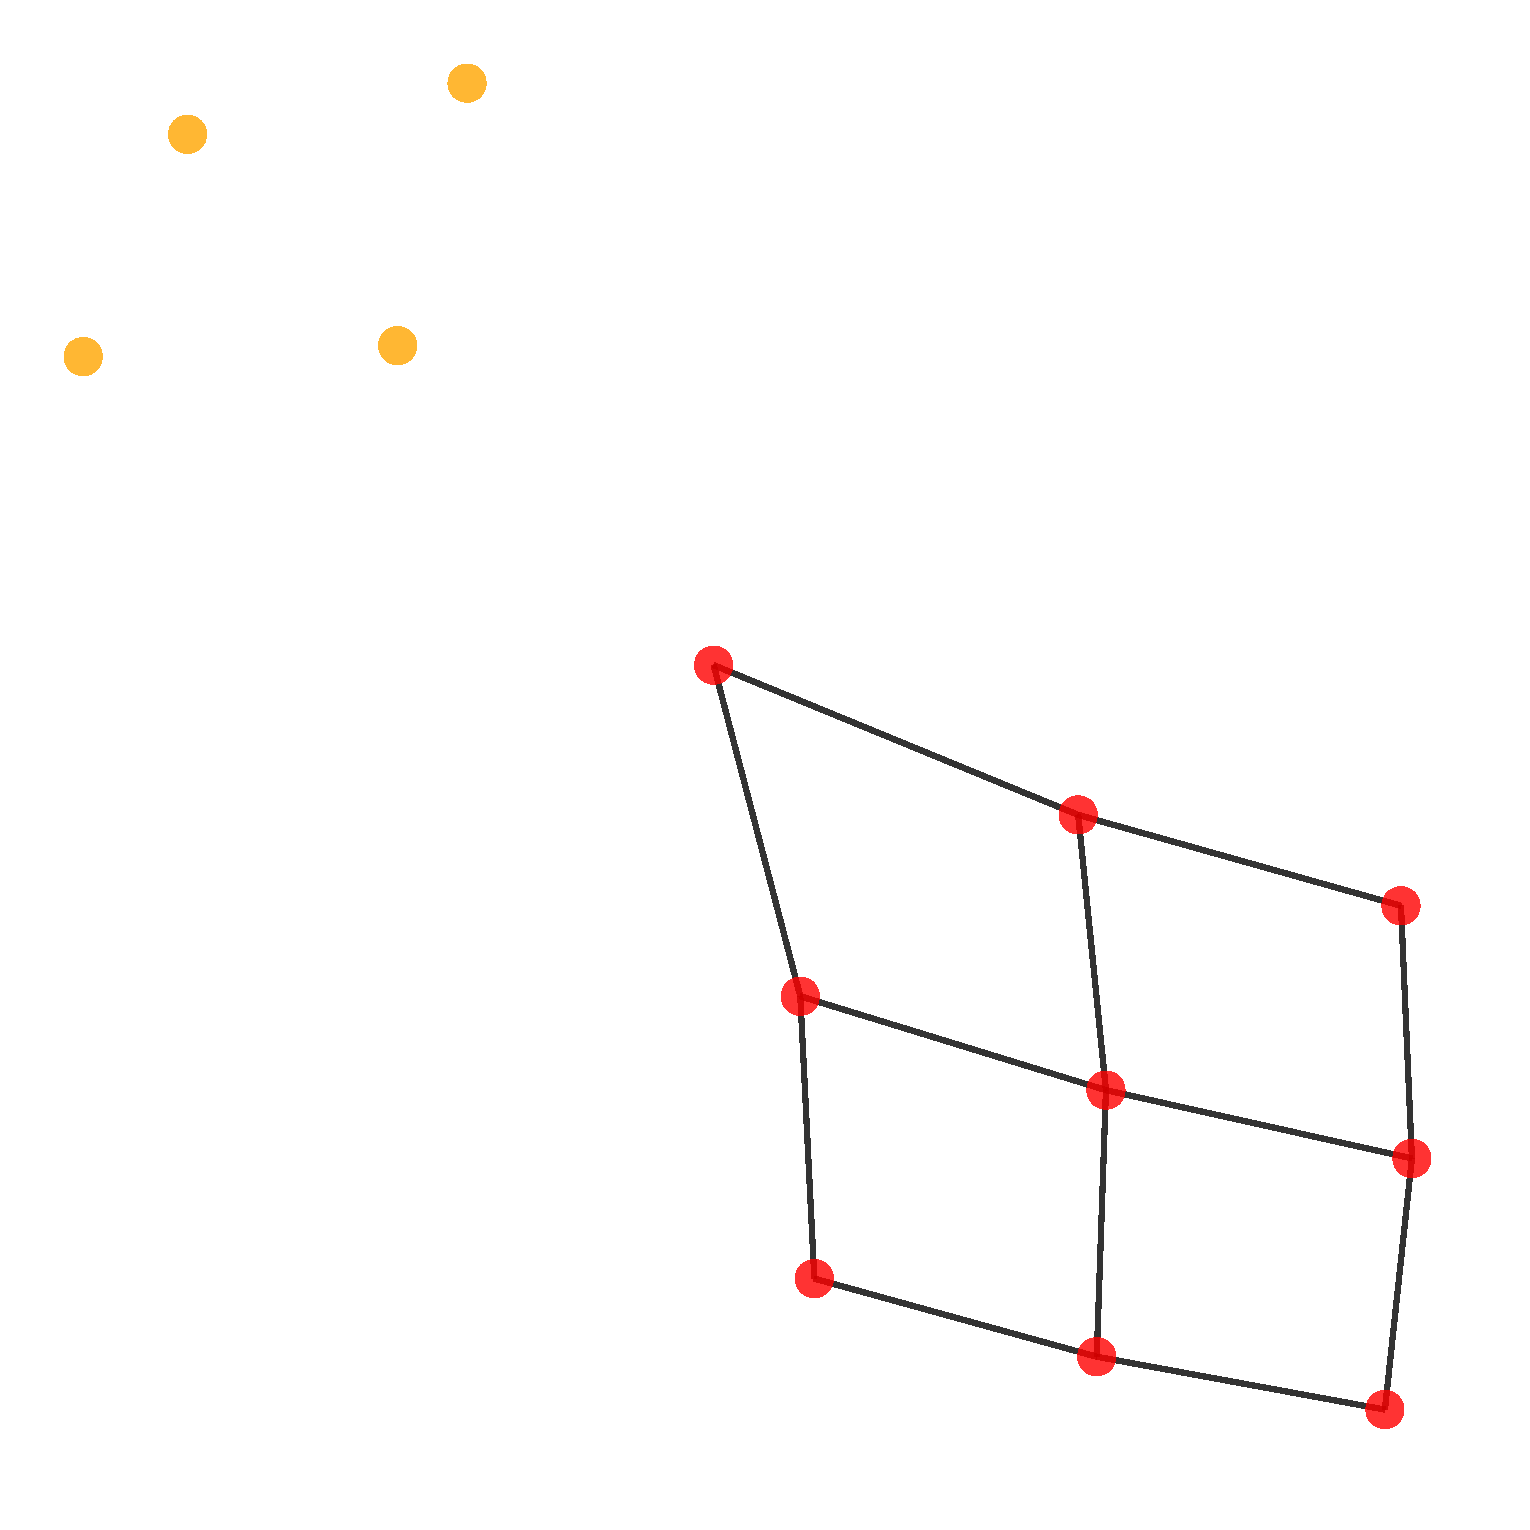
\includegraphics[width=\linewidth]{img/Tree-Grid/graph_2_explanation.pdf}
        \caption{\scriptsize Tree-Gr.}
        \label{fig:qual_grid}
    \end{subfigure}
    \begin{subfigure}[b]{0.15\textwidth}
        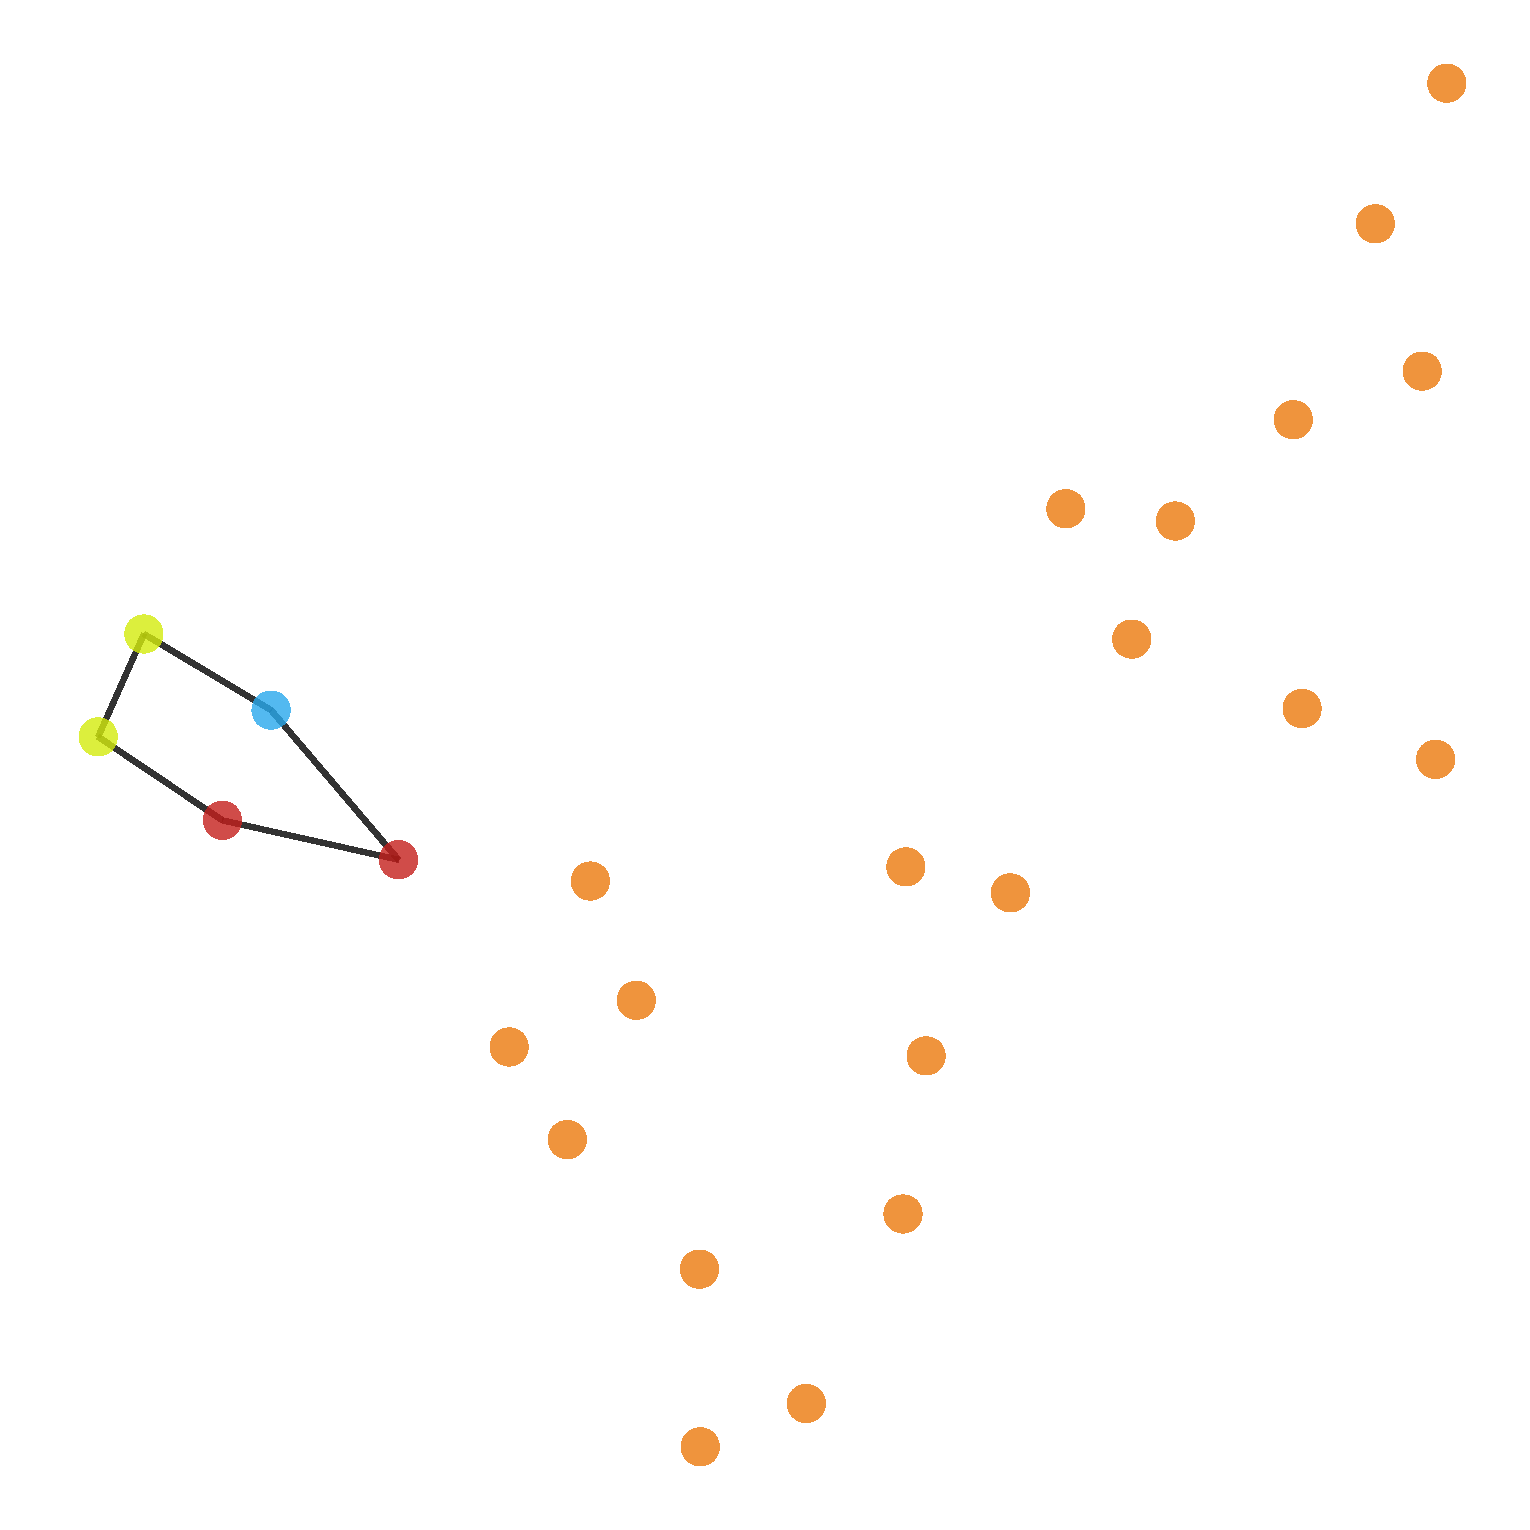
\includegraphics[width=\linewidth]{img/BA-2Motif/graph_3_explanation.pdf}
        \caption{\scriptsize BA-2M.}
        \label{fig:qual_2M}
    \end{subfigure}
    \begin{subfigure}[b]{0.15\textwidth}
        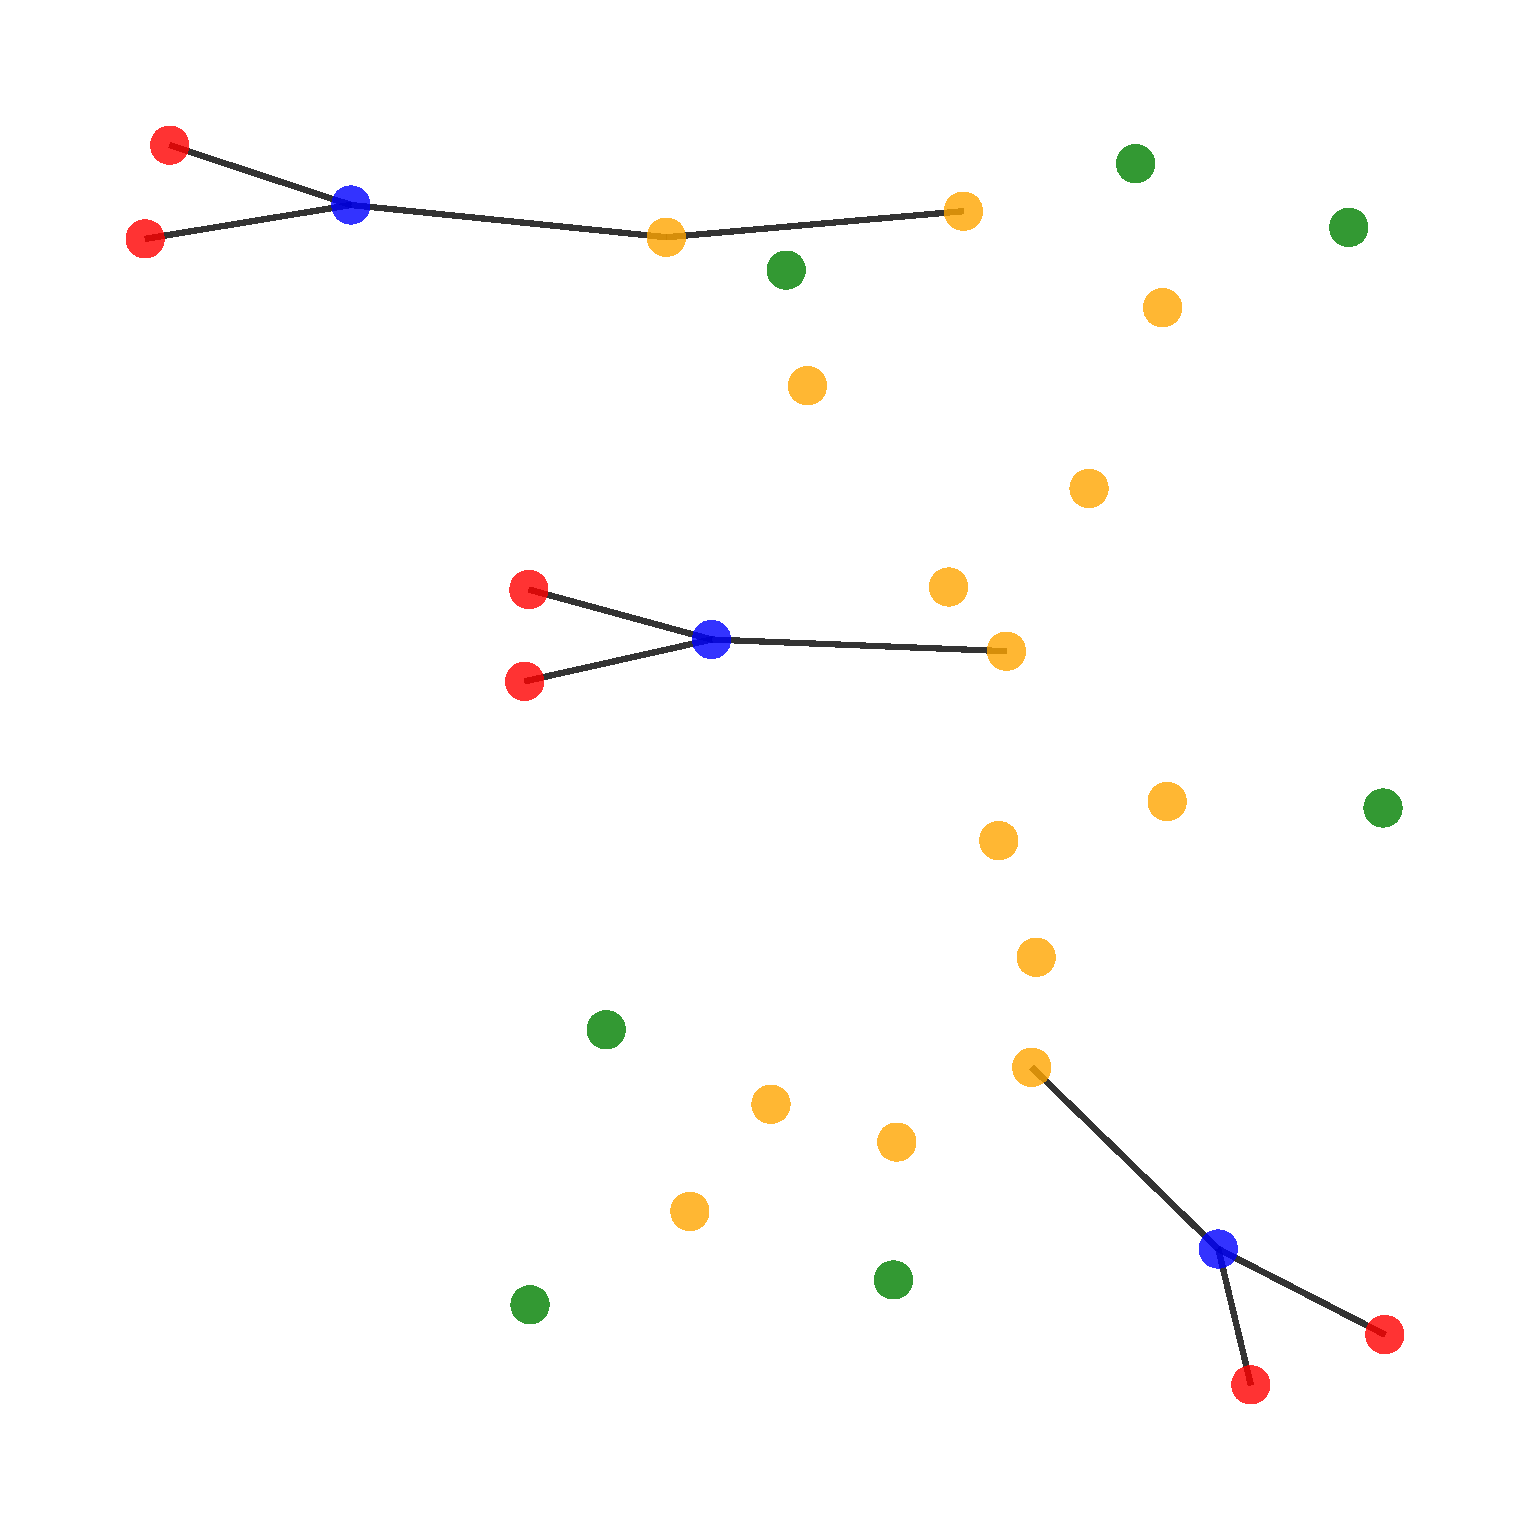
\includegraphics[width=\linewidth]{img/MUTAG/graph_12_explanation.pdf}
        \caption{\scriptsize MUTAG}
        \label{fig:qual_MUTAG}
    \end{subfigure}
    
    \caption{Explanations for one instance of each dataset.}
    \label{fig:qual_expl}
\end{figure}


%\subsection{Training on ALL instances - Evaluation only on motif instances?}
%This probably would not grant any insights, since training on non motif nodes should in theory mostly lead to all edges being irrelevant for prediction?? Bascially most edge could be removed and in theory the prediction of the node should not change at all, therefore no information can be gather from this?

%\textbf{Experimental setup}

%\textbf{Results}

\section{Generating Bipartite Explanations for NeuroSAT}
\label{sec:SAT-experiments}

In this section we present the experiments for generating bipartite explanations for unsatisfiable SAT problems evaluated by NeuroSAT \cite{selsam2018learning}. We describe the general procedure in Section \ref{sec:SAT-exp-setup}, followed by the results using the PGExplainer with a soft constraint in Section \ref{sec:sat-soft-exp}, as well as the hard constraint experiment in Section \ref{sec:sat-hard-exp}.

\subsection{Common Experimental Setup}
\label{sec:SAT-exp-setup}

NeuroSAT \cite{selsam2018learning} uses a distribution $\textbf{SR}(n)$ that creates pairs of SAT problems on $n$ variables, which are satisfiable and unsatisfiable, only differing in a singular negated literal. These are created by randomly sampling subclauses of $k$ variables, where each variable is negated with a probability of $50\%$. These subclauses are added to the problem until a SAT solver \cite{een2003extensible} finds it to be unsatisfiable. We adapt this to only contain singular unsatisfiable problems, rather than pairs of problems, since unsatisfiable cores only appear in unsatisfiable problems. The difficulty of the problems is slightly reduced by using $n=8$, to allow for the explainer to run on NeuroSAT on our limited hardware. We create a dataset of 100 problems.

We create the expected \ac{GT} with the deletion-based MUS extractor \lstinline|MUSX| from PySAT \cite{imms-sat18}, as described in section \ref{sec:Application_to_NeuroSAT}.

The quantitative evaluation is adopted from Section \ref{sec:PGE_exp_setup}, with the positive targets being the edges that appear in the corresponding \ac{GT} MUS of each problem. We additionally evaluate the test instance that achieves the highest individual AUROC score and visualize it. Since the qualitative evaluation relies on knowing $k$, we calculate this dynamically during evaluation from the \ac{GT} of the current problem. Clause nodes are drawn in red, while nodes representing literals are drawn in magenta.

The NeuroSAT model trained on a $\textbf{SR}(40)$ distribution was provided by a fellow student. It achieves an accuracy of 1.0 on the dataset we created.

We apply PGExplainer in the inductive setting, using a 50/25/25 split for training, evaluating and testing the NeuroSAT explainer. \bigskip

\textbf{Hyperparameter Search}\par
We perform a hyperparameter search for both the explainer with the soft constraint, and the explainer with the applied hard constraint. We follow the general grid search procedure used for the previous experiments, but introduce 4 new hyperparameters, 1 exclusive to the hard constraint and 2 exclusive to the soft constraint. $\alpha_{arch} \in \{0,1\}$, exclusive to the hard constraint, denotes whether a more complex MLP architecture is used in the explainer. The second introduced hyperparameter $\alpha_{concat} \in \{0,1\}$ controls whether the node embeddings $\mathbf{z}$ are used from the last iteration of NeuroSAT or if a concatenation of the states at multiple iterations shall be used (see Section \ref{sec:NeuroSAT_extension}). For the soft constraint, we also try using the AdamW \cite{loshchilov2017decoupled} optimizer from PyTorch with an internal weight decay of $0.01$, denoted by $\alpha_{AdamW} \in \{0,1\}$. Lastly, the coefficient $\alpha_{c} \in \mathbb{R}^+$ controls the effect of the soft constraint $R_C$ (see Equation \ref{eq:soft_restraint}) on the loss. This is disregarded in the hard constraint experiment, as the hard constraint replaces the soft constraint. The sample bias $b$ used in PGExplainer is disregarded completely. We evaluate the search with respect to the validation AUROC score, as well as the validation loss. The specification of both grid searches can be found in Appendix \ref{sec:neurSAT_sweeps}.


\subsection{Soft Constraint Experiment}
\label{sec:sat-soft-exp}
\textbf{Experimental Setup}\par
In this experiment we apply the soft constraint introduced in Section \ref{sec:NeuroSAT_extension} to the PGExplainer to generate explanations for unsatisfiable SAT problems learned from NeuroSAT predictions. After performing the grid search, we utilize the optimal parameters to evaluate the test AUROC over 10 seeded runs. Additionally, we provide qualitative explanations in comparison to the \ac{GT} MUS for the problem that results in the highest individual AUROC. \bigskip

\textbf{Results}\par
We found that the grid search resulted in a maximum average validation AUROC of 0.5248 and a minimal score of 0.4726. This can be seen in Figure \ref{fig:soft-sweep}. All runs achieved results in this interval, indicating completely random edge predictions on average. It seems that regardless of the tested hyperparameters the general explanations of unsatisfiable problems, as learned from NeuroSAT, do not align with unsatisfiable cores.

We note that a low size regularization has the highest impact on the mean AUROC score, since a high value leads to uniform edge importance scores of 0. This is followed by a high consistency regularization, as well as a low learning rate. The other hyperparameters are not as decisive. We select the hyperparameter combination that maximizes the validation AUROC, as highlighted in Table \ref{tab:sweep_conf_soft}. \bigskip

The mean test AUROC score achieved over 10 runs is listed in Table \ref{tab:res_neuroSAT}.

Over all runs, the highest individual test AUROC score of 0.711 is achieved for seed 4 (see Figure \ref{fig:soft_quant}). As seen in Figure \ref{fig:soft_shared}, only 2 edges are identified correctly and no full clause is predicted. Since this does not correspond with the relatively high AUROC score, we stress that the AUROC might not be an ideal metric for evaluation in this context. Nevertheless, we did not find a visualization that shared significantly more edges with its \ac{GT} or indicated a better learning of the MUS motif.

\begin{figure}[h]
    \centering
    % First 3 images
    \begin{subfigure}[b]{0.3\textwidth}
        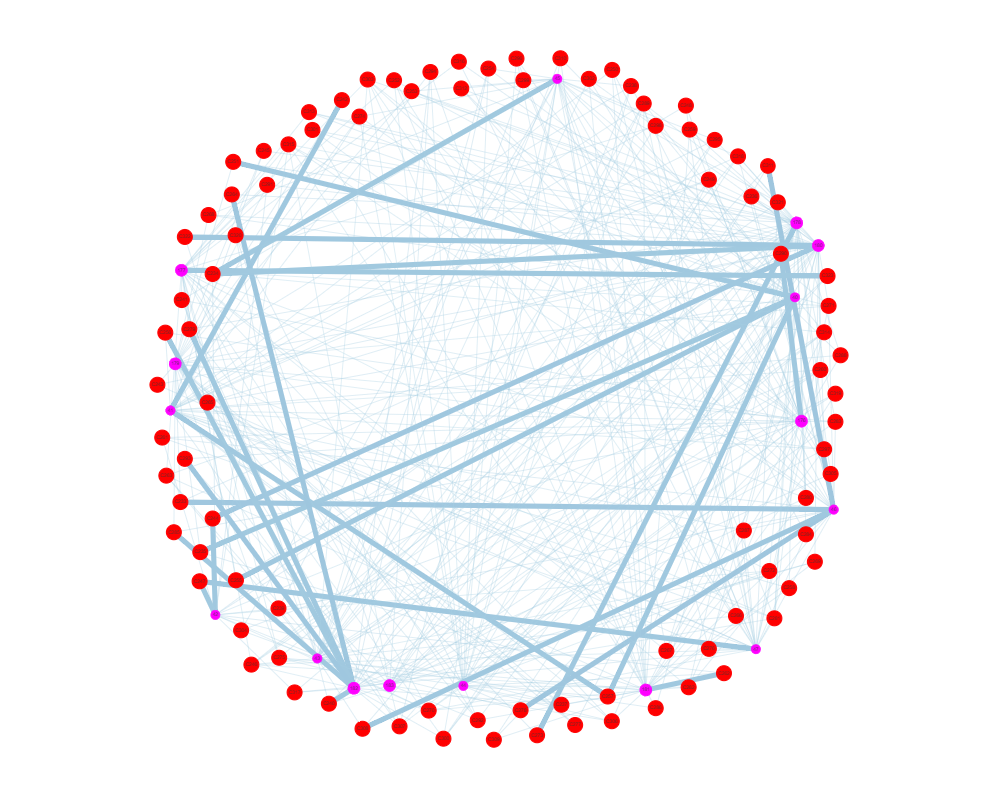
\includegraphics[width=\linewidth]{img/SAT-soft/2025-05-14 20_50_23-seed4_highestAUC_TEST.html.png}
        \caption{Soft explanation}
        \label{fig:soft_pred}
    \end{subfigure}
    \begin{subfigure}[b]{0.3\textwidth}
        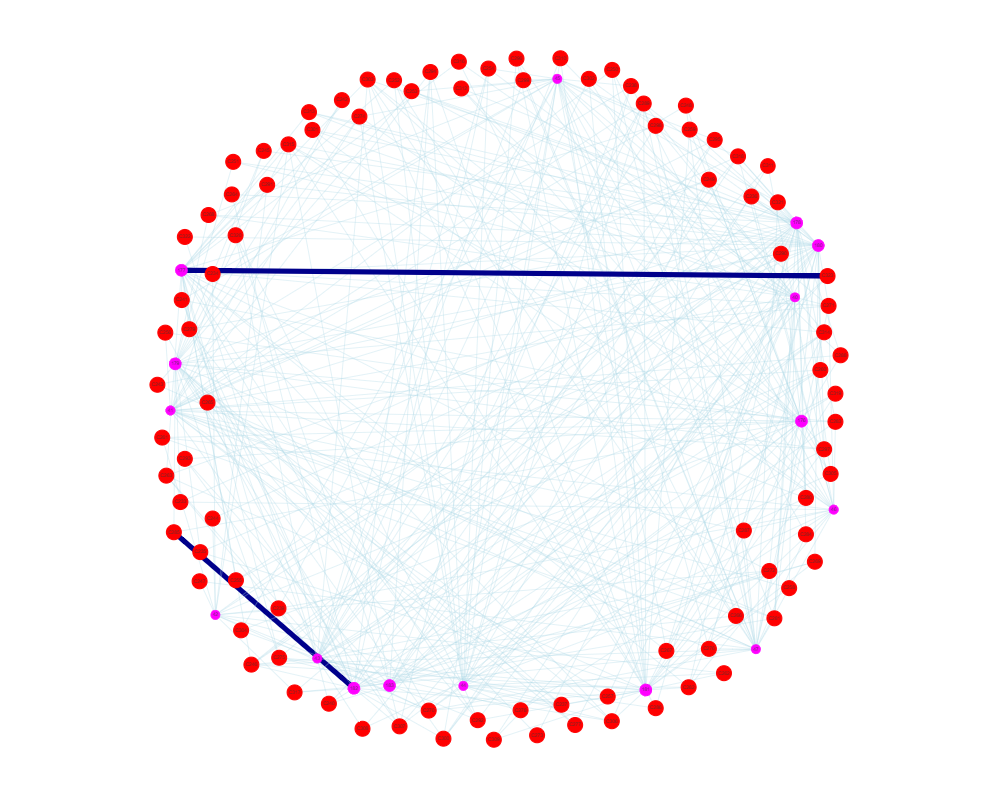
\includegraphics[width=\linewidth]{img/SAT-soft/2025-05-14 20_51_51-seed4_highestAUC_commonEdges_TEST.html.png}
        \caption{Common edges}
        \label{fig:soft_shared}
    \end{subfigure}
    \begin{subfigure}[b]{0.3\textwidth}
        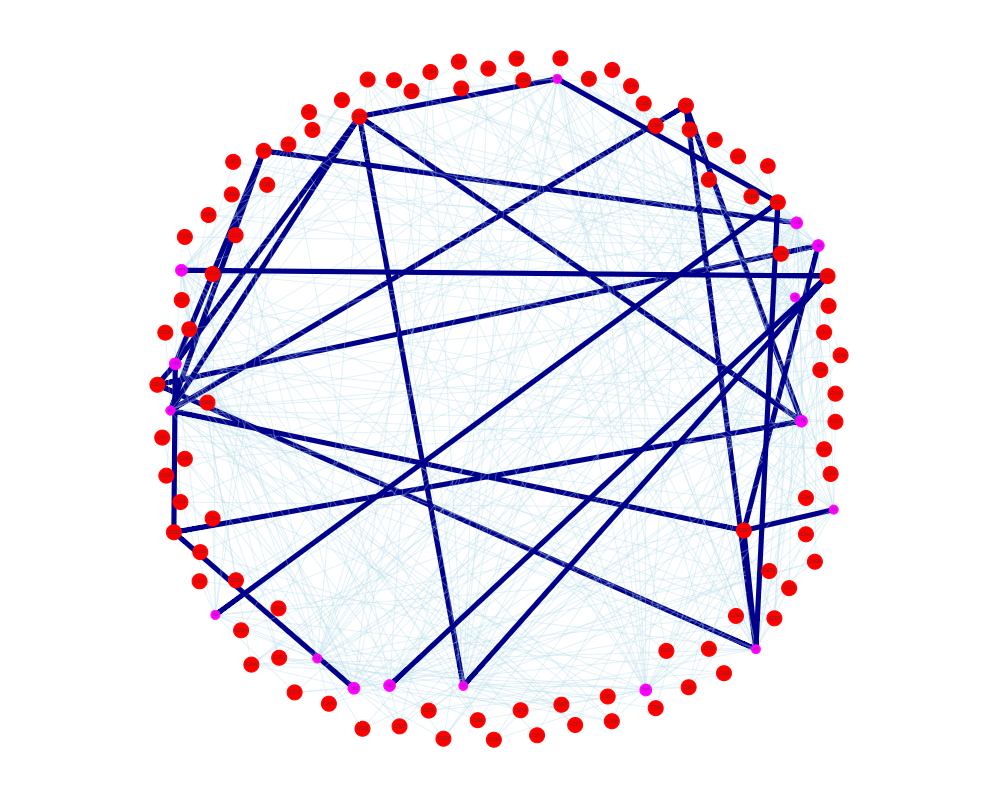
\includegraphics[width=\linewidth]{img/SAT-soft/2025-05-14 20_52_03-seed4_highestAUC_gt_TEST.html.png}
        \caption{\ac{GT}}
        \label{fig:soft_gt}
    \end{subfigure}
    \caption[Visualization of soft constraint explanation]{Visualization of the soft constraint explanation that achieves the highest individual test AUROC score when compared to its corresponding \ac{GT} unsatisfiable core.}
    \label{fig:soft_quant}
\end{figure}

\subsection{Hard Constraint Experiment}
\label{sec:sat-hard-exp}
\textbf{Experimental Setup}\par
In this experiment we apply the hard constraint introduced in Section \ref{sec:NeuroSAT_extension} to the PGExplainer to generate explanations for unsatisfiable SAT problems learned from NeuroSAT predictions. The experimental setup is adopted from Section \ref{sec:sat-soft-exp}. \bigskip

\textbf{Results}\par
The grid search revealed that none of the parameter configurations achieves an AUROC score above $0.5$ and below $0.44$. Since $0.5$ equals random guessing and is usually caused by all edges being predicted with a uniform score of 0, we select the hyperparameter combination that achieves the highest score, while maintaining edge weights unequal to 0. We found that a low learning rate is important to keep the edge predictions from reaching 0, as these steadily decrease over training time. $\alpha_s=1.0$ further enhanced this unwanted behavior. The resulting combination used for the experiment is highlighted in Table \ref{tab:sweep_conf_hard}. \bigskip

Using a concatenation of the embeddings at multiple iterations achieved worse results than the usual graph task procedure when considering the highest individual AUROC of a validation instance. However, this does not consider whether a general procedure is learned. It is important to note that the average of the lowest absolute edge importance score per run is 0.34, while the average of the highest score is 0.44. This indicates a reasonable span of importance scores, but may still lack in the sense of resembling approximated discrete masks.\bigskip

We found that the run on seed 0 achieves the highest individual test AUROC of 0.776 (See Figure \ref{fig:hard_quant}). It is notable that 2 out of 6 full clauses are predicted correctly. Nevertheless, the mean test AUROC only sees a slight increase as presented in Table \ref{tab:res_neuroSAT}. \bigskip

We present an additional evaluation of the satisfiability of an explanation in Appendix \ref{sec:sat_expl_hard_cons}. \bigskip

\begin{table}[ht]
    \centering
    \scriptsize
    \begin{tabularx}{0.35\textwidth}{l*{1}{X}}   % Adjust width as needed
    \toprule
    \textbf{Method} & \textbf{AUROC} \\
    \midrule
    Soft Constraint & 0.512$\pm$0.023 \\
    \midrule
    Hard Constraint & 0.528$\pm$0.013 \\
    \bottomrule
    \end{tabularx}
    \caption[Inductive performance of explainer on NeuroSAT]{Explanation AUROC for NeuroSAT predictions of unsatisfiable SAT problems.}
    \label{tab:res_neuroSAT}
\end{table}

\begin{figure}[h]
    \centering
    % First 3 images
    \begin{subfigure}[b]{0.3\textwidth}
        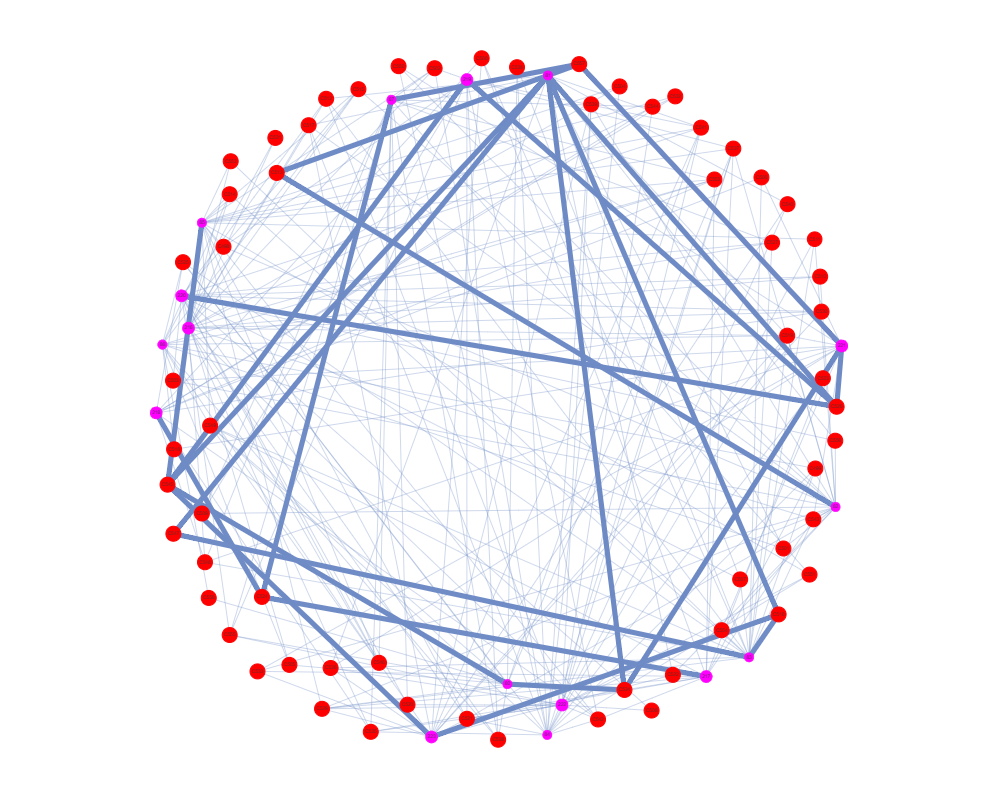
\includegraphics[width=\linewidth]{img/SAT-hard/2025-05-14 20_53_31-seed0_highestAUC_TEST.html.png}
        \caption{Hard explanation}
        \label{fig:hard_pred}
    \end{subfigure}
    \begin{subfigure}[b]{0.3\textwidth}
        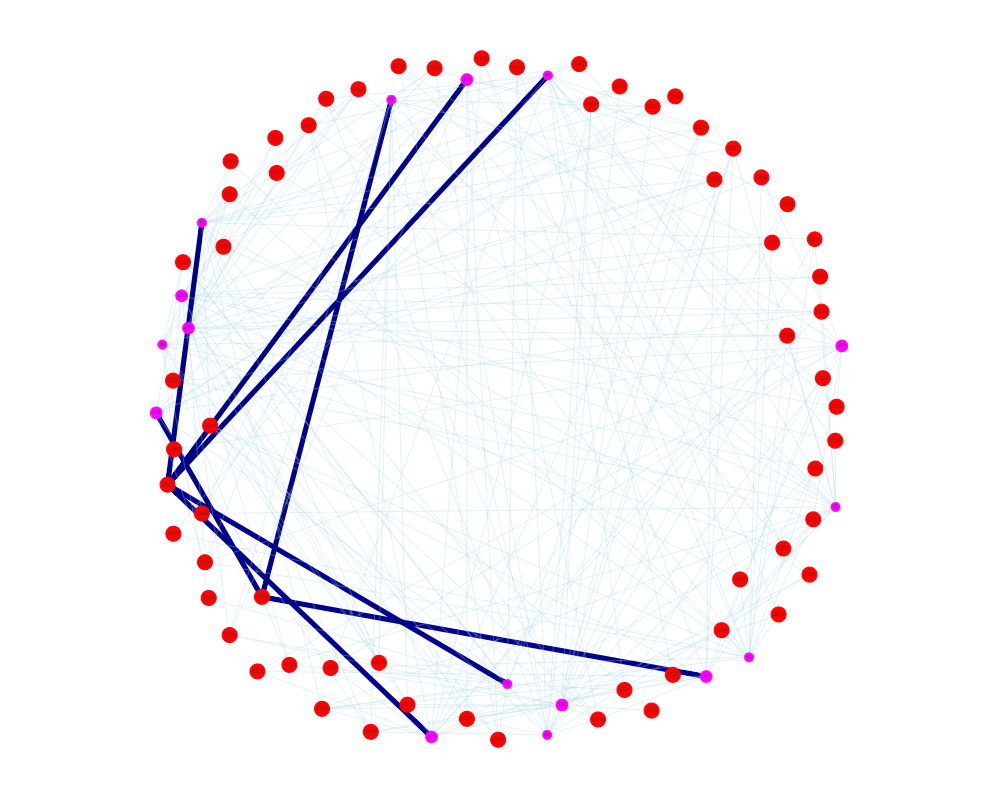
\includegraphics[width=\linewidth]{img/SAT-hard/2025-05-14 20_53_47-seed0_highestAUC_commonEdges_TEST.html.png}
        \caption{Common edges}
        \label{fig:hard_shared}
    \end{subfigure}
    \begin{subfigure}[b]{0.3\textwidth}
        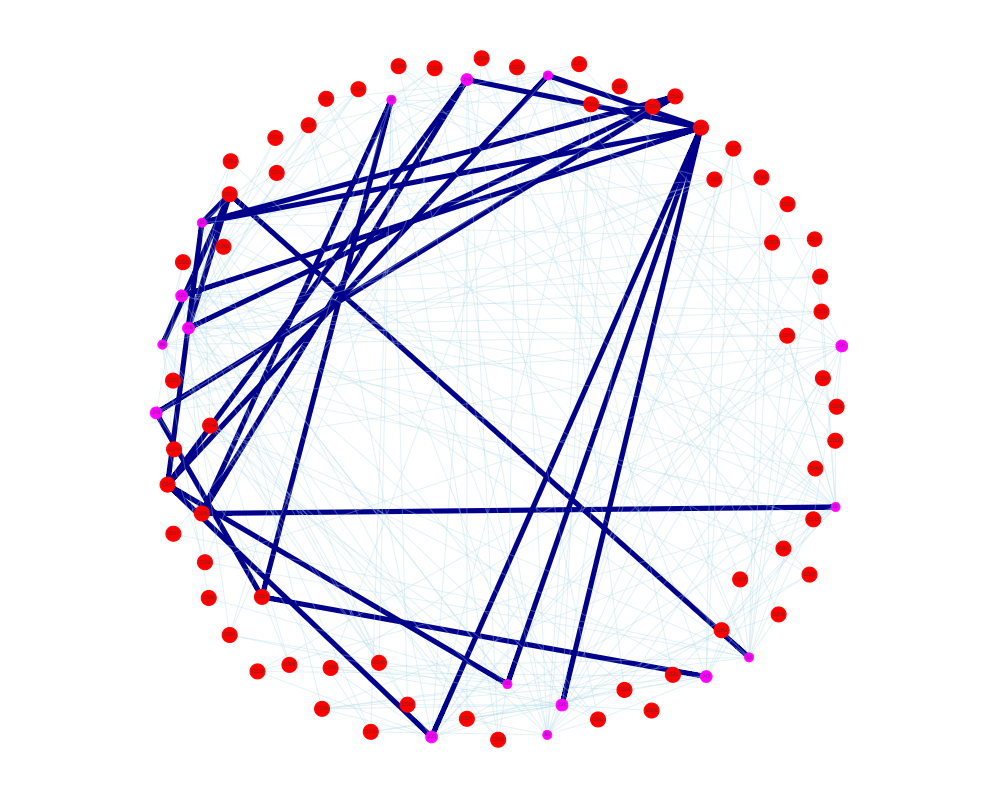
\includegraphics[width=\linewidth]{img/SAT-hard/2025-05-14 20_53_57-seed0_highestAUC_gt_TEST.html.png}
        \caption{\ac{GT}}
        \label{fig:hard_gt}
    \end{subfigure}
    \caption[Visualization of hard constraint explanation]{Visualization of the hard constraint explanation that achieves the highest individual test AUROC score when compared to its corresponding \ac{GT} unsatisfiable core.}
    \label{fig:hard_quant}
\end{figure}

Furthermore, we found that running the training on a singular seed for 500 epochs resulted in a converging loss, as well as a converging metric score close to $0.46$. A local score minimum is reached in epoch 60 with a value of $0.44$. Since this is very close to a score indicating randomness, we conclude that the post-hoc explanations provided by our modified version of PGExplainer for NeuroSAT do not align with MUSes.
